\documentclass[11pt]{article}
\usepackage[utf8]{inputenc}
\usepackage[T1]{fontenc}
\usepackage[spanish,es-nodecimaldot]{babel}
\usepackage[a4paper,margin=2.2cm]{geometry}
\usepackage{amsmath,amssymb,booktabs,array,longtable,graphicx,float,caption,hyperref,xcolor,fancyhdr,multicol}
\usepackage{enumitem}
\graphicspath{{figures/}}
\hypersetup{colorlinks=true,linkcolor=black,urlcolor=blue,citecolor=black}
\setlist[itemize]{topsep=3pt,itemsep=2pt,parsep=0pt,leftmargin=1.2em}
\setlist[enumerate]{topsep=3pt,itemsep=2pt,parsep=0pt,leftmargin=1.4em}
\definecolor{navy}{HTML}{1B263B}
\definecolor{softblue}{HTML}{E8F1FA}
\definecolor{softgreen}{HTML}{EAF6F0}
\definecolor{softorange}{HTML}{FFF4E5}
\definecolor{softpurple}{HTML}{F4ECFA}
\definecolor{linegray}{HTML}{D0D7DE}
\definecolor{darkgray}{HTML}{37474F}
\pagestyle{fancy}
\fancyhf{}
\lhead{Reporte final }
\rhead{Mapper/TDA de exoplanetas}
\cfoot{\thepage}
\renewcommand{\headrulewidth}{0.4pt}
\setlength{\headheight}{14pt}
\setlength{\parskip}{0.55em}
\setlength{\parindent}{0pt}
\captionsetup{font=small,labelfont=bf}

\newcommand{\executivebox}[2]{%
\begin{center}
\fcolorbox{navy}{#1}{\begin{minipage}{0.92\textwidth}\vspace{0.55em}#2\vspace{0.55em}\end{minipage}}
\end{center}}
\newcommand{\metric}[2]{\begin{tabular}{@{}c@{}}\Large\textbf{#1}\\[-1pt]\small #2\end{tabular}}
\newcommand{\code}[1]{\texttt{#1}}

\title{\vspace{-1.0cm}\textbf{Priorización topológica de incompletitud observacional en catálogos de exoplanetas}\\[0.3em]\large De sesgos de descubrimiento a rankings observacionales interpretables}
\author{Proyecto Mapper/TDA de exoplanetas}
\date{Versión ejecutiva final}

\begin{document}
\maketitle

\executivebox{softblue}{\textbf{Resultado central.} El proyecto transforma sesgos de descubrimiento en una herramienta de priorización observacional basada en estructura topológica, estabilidad local y soporte físico-orbital. La salida final es un ranking de regiones Mapper y planetas ancla donde el catálogo parece topológicamente incompleto, con una lectura ordenada para inspección futura.}

\begin{center}
\begin{tabular}{@{}llll@{}}
\toprule
\textbf{Capa} & \textbf{Resultado } & \textbf{Caso principal} & \textbf{Lectura} \\
\midrule
Región & Prioridad regional por TOI & \code{cube12\_cluster0} & región más informativa \\
Ancla exploratoria & Ranking ATI original & HIP 97166 c & señal local sensible a escala \\
Ancla conservadora & Ranking ATI conservador & HIP 90988 b & caso final más defendible \\
Transición Mapper & Membresía múltiple & HD 42012 b & frontera entre vecindarios \\
Soporte secundario & Déficit estable alternativo & HD 4313 b & candidato complementario \\
\bottomrule
\end{tabular}
\end{center}

\tableofcontents
\newpage

\section{Resumen }

El proyecto evolucionó desde una auditoría de sesgos observacionales hasta una metodología completa de priorización topológica. El resultado final integra cinco capas: datos imputados y trazables, grafos Mapper comparables, auditoría por método de descubrimiento, sombra observacional local y validación multiescala de anclas. La contribución ejecutiva es clara: convertir una propiedad conocida del catálogo --su heterogeneidad observacional-- en una señal estructurada para decidir qué regiones merecen inspección adicional.

\begin{figure}[H]
\centering
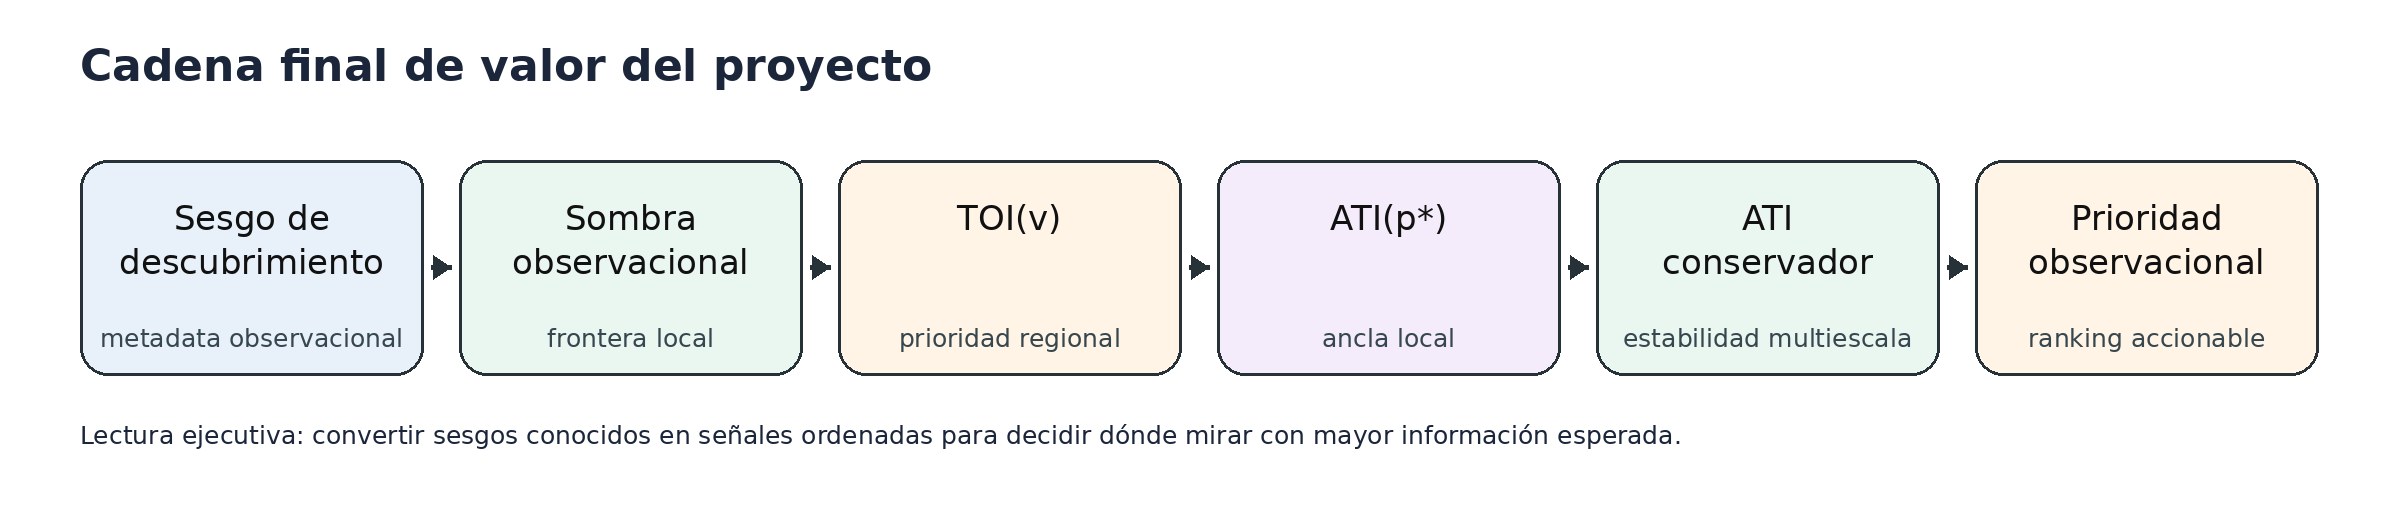
\includegraphics[width=0.98\textwidth]{fig01_pipeline_chain.png}
\caption{Cadena final de valor del proyecto. La secuencia convierte sesgo de descubrimiento en prioridad observacional mediante sombra local, TOI regional, ATI local y una versión conservadora que favorece estabilidad multiescala.}
\end{figure}

\executivebox{softgreen}{\textbf{Conclusión principal.} TOI/ATI prioriza regiones Mapper y planetas ancla donde el catálogo parece topológicamente incompleto, ofreciendo una ruta ordenada para inspección observacional futura.}

La lectura final se apoya en cuatro resultados medibles. Primero, el pipeline de imputación generó una matriz completa para las siete variables principales, preservando trazabilidad entre valores observados, derivados e imputados. Segundo, Mapper produjo una familia de grafos donde el espacio orbital emergió como el candidato estructural más informativo: 124 nodos, 196 aristas, \(\beta_1=96\) e imputación media nodal cercana a 0.011. Tercero, la auditoría de método mostró que la topología contiene una señal observacional fuerte, especialmente ligada a tránsito y velocidad radial. Cuarto, la capa TOI/ATI transformó esa señal en rankings interpretables, cerrando con una validación conservadora que desplaza el caso final hacia HIP 90988 b.

\section{Glosario  y notación}

\begin{longtable}{p{0.22\textwidth}p{0.72\textwidth}}
\toprule
\textbf{Término} & \textbf{Definición operacional} \\
\midrule
Mapper & Grafo topológico construido con cubiertas solapadas del espacio de lentes y clusters locales. Cada nodo representa una comunidad local de planetas. \\
Nodo \(v\) & Región local del grafo Mapper con conjunto de planetas \(S_v\). Por solapamiento, un planeta puede aparecer en más de un nodo. \\
Sombra observacional & Señal local donde un nodo difiere de sus vecinos en composición por método, con baja mezcla, baja imputación y soporte de tamaño. \\
\(R^3\) físico-orbital & Espacio \((\log M_p,\log P,\log a)\), usado para comparar masa planetaria, periodo orbital y semieje mayor. \\
TOI\((v)\) & \textit{Topological Observational Incompleteness}: prioridad regional de un nodo Mapper. \\
ATI\((p^*)\) & \textit{Anchor Topological Incompleteness}: prioridad local de un planeta ancla \(p^*\). \\
ATI conservador & Variante interpretativa que penaliza sensibilidad al radio y favorece déficits locales estables. \\
Prioridad observacional & Ranking final de anclas donde observaciones futuras o modelos de completitud tendrían mayor valor informativo. \\
\bottomrule
\end{longtable}

\section{La base reproducible: imputación trazable y cobertura Mapper}

La primera contribución del proyecto fue construir una base de datos apta para Mapper sin borrar la procedencia de los valores. El pipeline comparó imputación por mediana, KNN e \textit{IterativeImputer}; la versión visualizada y usada para los resultados principales fue \textit{iterative}. La decisión se apoyó en validación enmascarada y en la necesidad de conservar una matriz completa para siete variables: radio, masa, densidad, periodo orbital, semieje mayor, insolación y temperatura de equilibrio.

\begin{figure}[H]
\centering
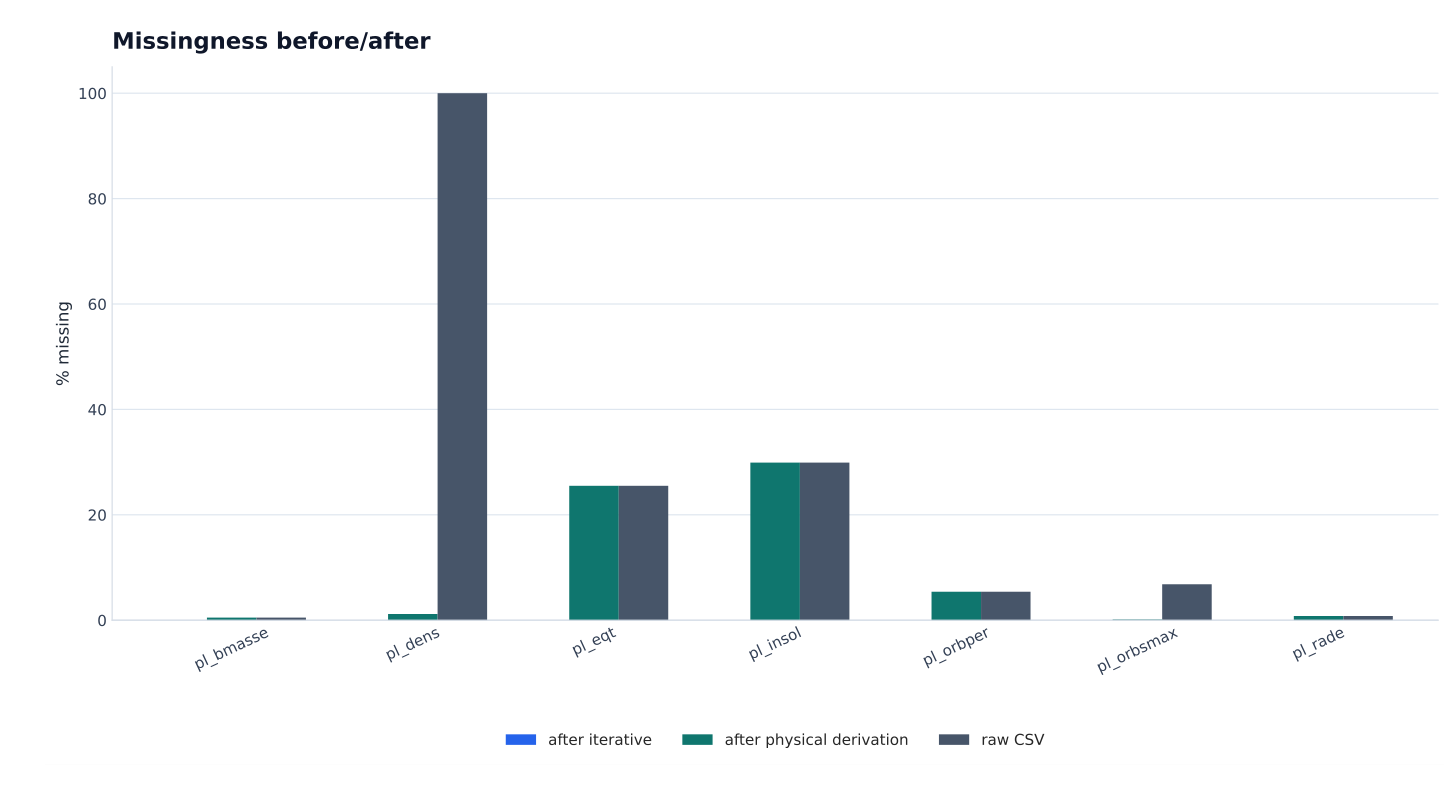
\includegraphics[width=0.88\textwidth]{fig02_missingness_before_after.png}
\caption{Reducción de faltantes antes y después de derivación física e imputación. La figura muestra la transición desde el CSV original hacia una matriz completa, diferenciando el valor de derivar físicamente antes de imputar estadísticamente.}
\end{figure}

\begin{figure}[H]
\centering
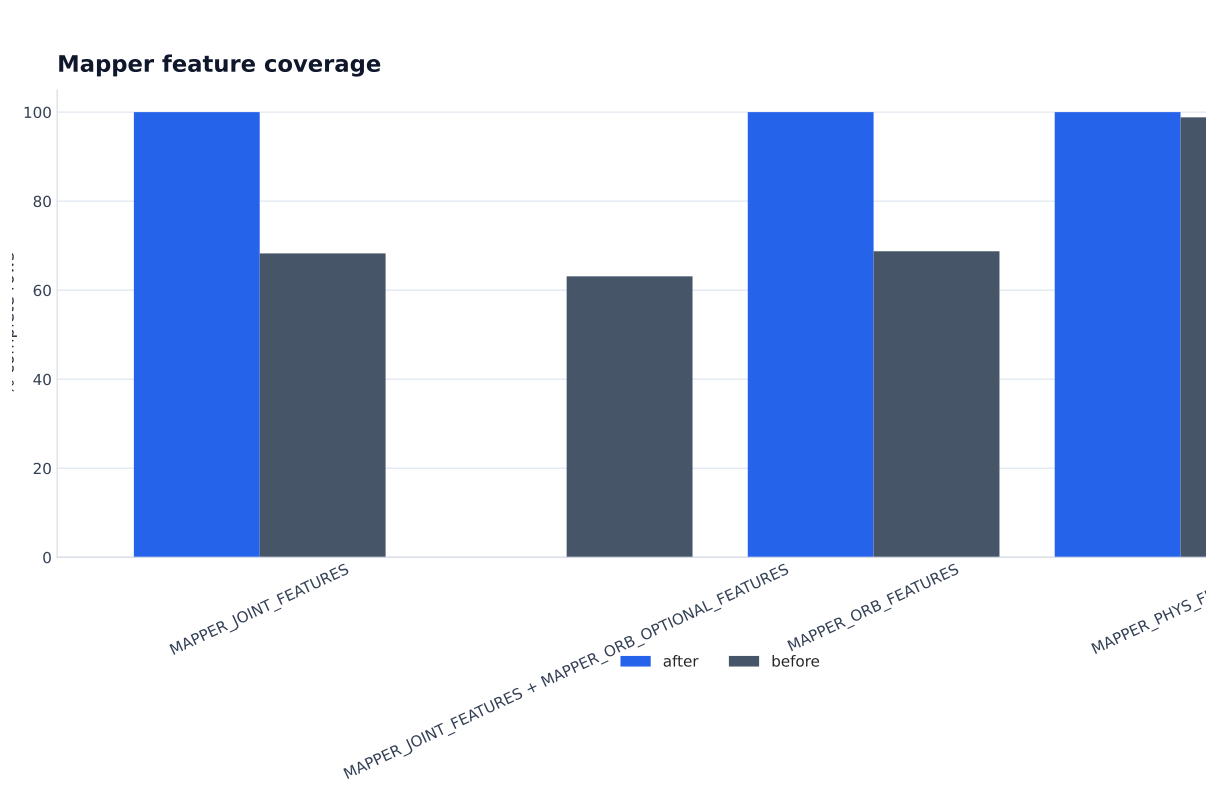
\includegraphics[width=0.78\textwidth]{fig03_mapper_coverage.png}
\caption{Cobertura de espacios Mapper antes y después del pipeline. El espacio conjunto de variables principales queda habilitado para análisis topológico completo, manteniendo banderas de trazabilidad para auditar la interpretación posterior.}
\end{figure}

El logro importante no fue solo llenar una tabla. Fue crear una matriz analítica donde cada valor conserva su historia: observado, derivado por relación física o imputado por modelo. Esa trazabilidad permitió que las etapas posteriores hablaran de regiones con baja o alta dependencia de imputación, en lugar de tratar todos los nodos como igualmente confiables.

\executivebox{softorange}{\textbf{Lectura ejecutiva.} La imputación funcionó como infraestructura científica: habilitó Mapper sobre todo el catálogo y, al mismo tiempo, dejó visible la procedencia de los valores que sostienen cada región.}

\section{Mapper como atlas topológico del catálogo}

La segunda etapa construyó una comparación entre espacios físicos, orbitales, térmicos y conjuntos. La lectura final favorece el espacio orbital porque combina complejidad topológica alta con dependencia baja de imputación. En lenguaje de negocio científico: es la zona donde el grafo ofrece más estructura útil con menor costo epistemológico.

\begin{figure}[H]
\centering
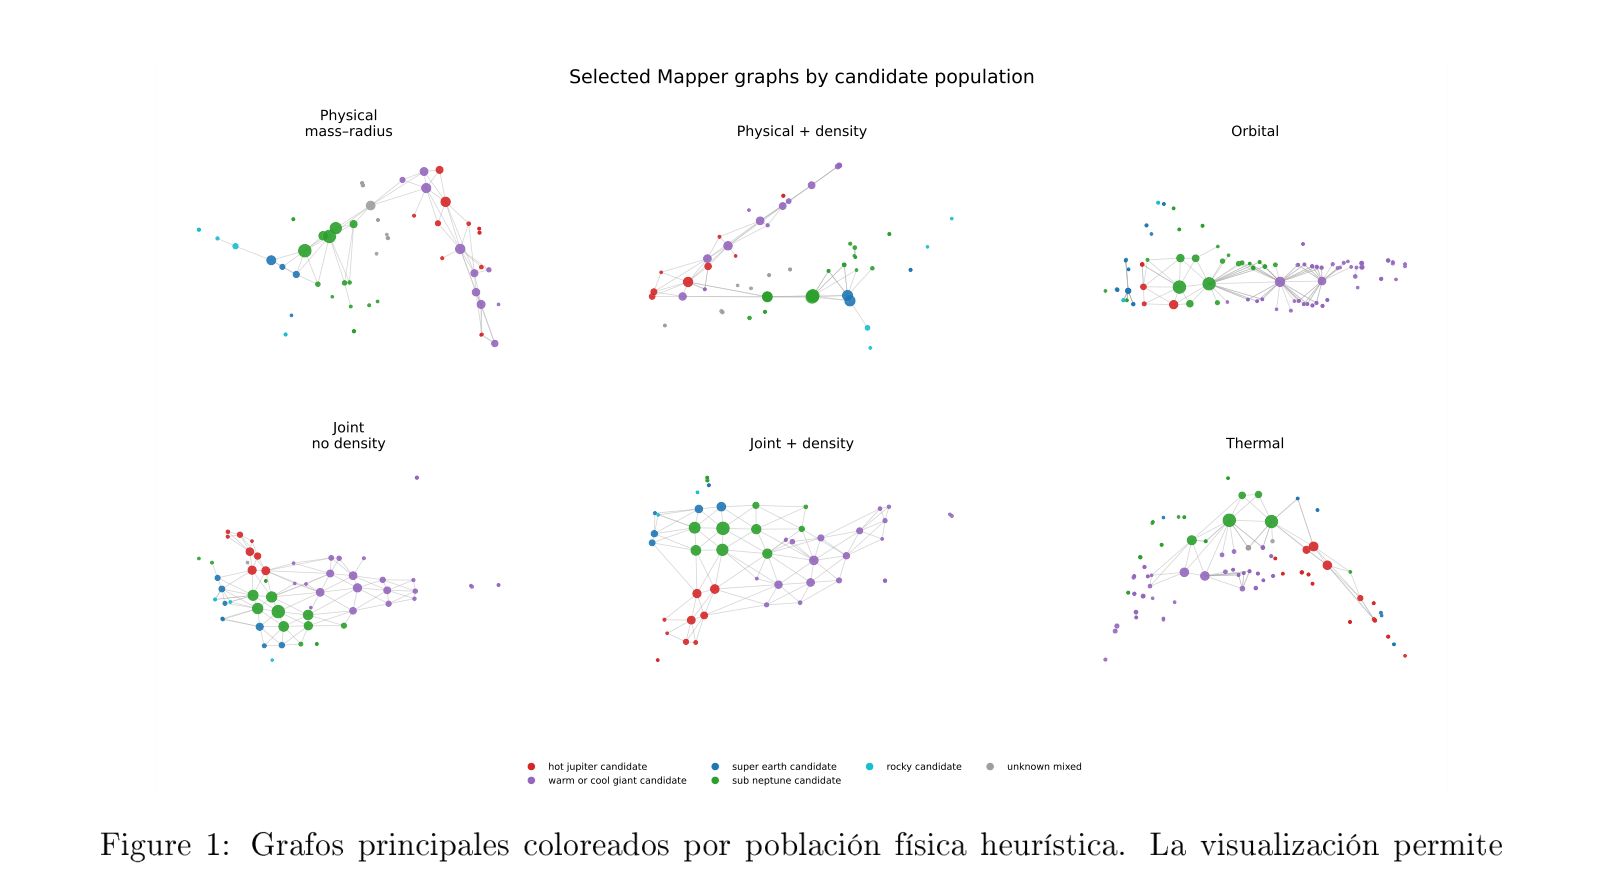
\includegraphics[width=0.98\textwidth]{fig04_mapper_candidate_population.png}
\caption{Grafos Mapper seleccionados coloreados por población candidata. La figura resume cómo distintos espacios de variables organizan el catálogo en regiones físicas, orbitales y térmicas interpretables.}
\end{figure}

\begin{figure}[H]
\centering
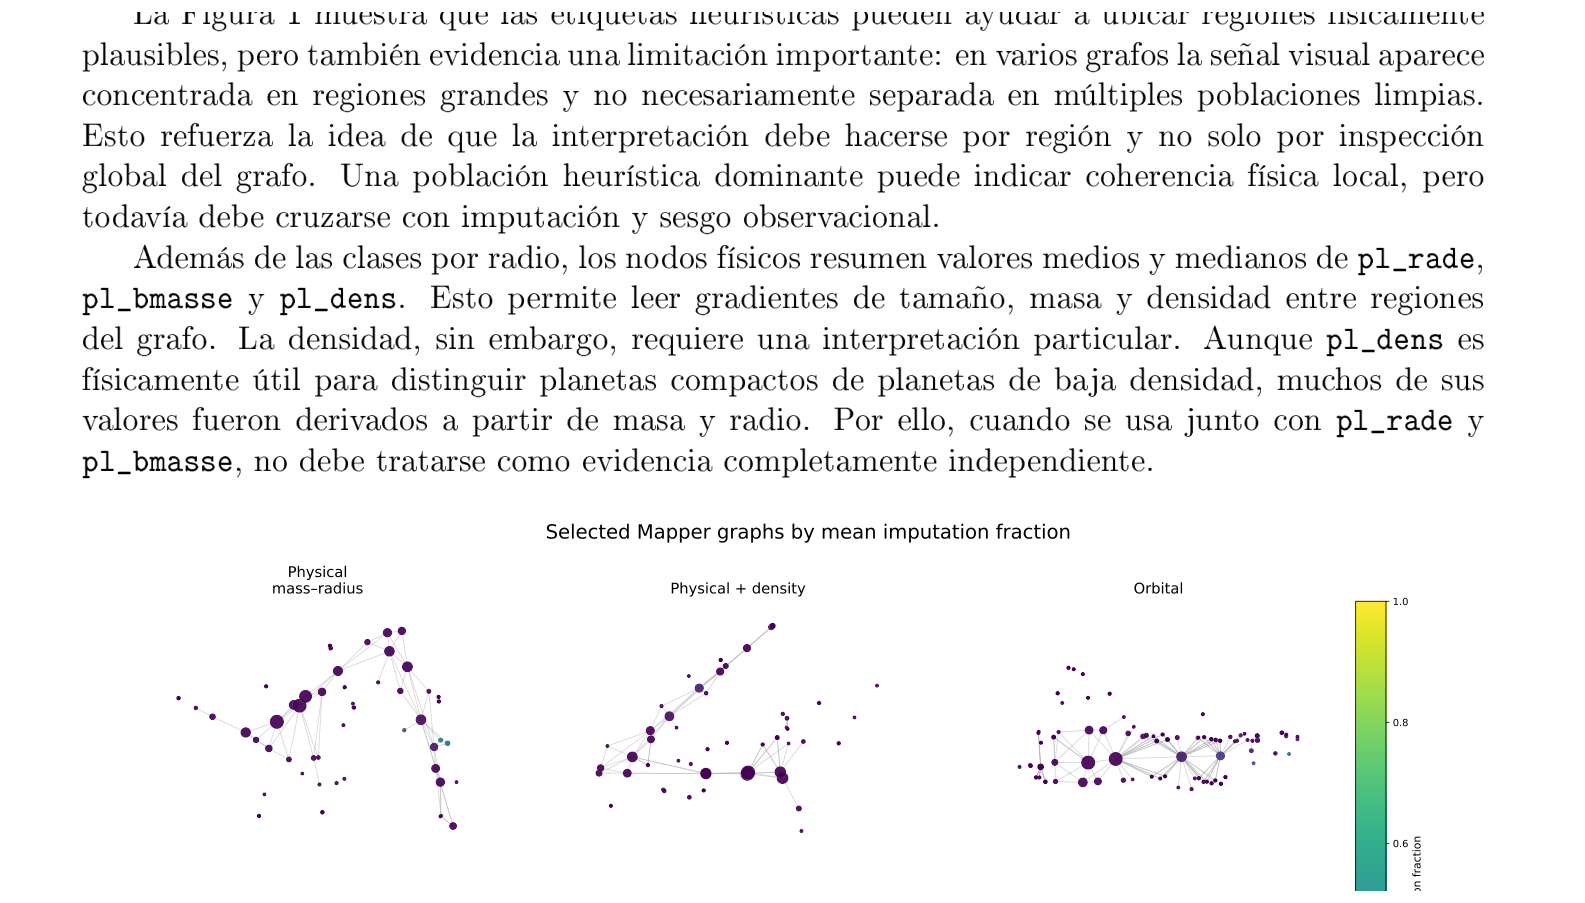
\includegraphics[width=0.96\textwidth]{fig05_mapper_imputation_fraction.png}
\caption{Grafos seleccionados coloreados por fracción media de imputación. La comparación separa estructura visualmente rica de estructura defendible; el espacio orbital destaca por baja imputación relativa frente al térmico.}
\end{figure}

\begin{center}
\renewcommand{\arraystretch}{1.25}
\begin{tabular}{@{}lrrrrl@{}}
\toprule
\textbf{Grafo} & \textbf{Nodos} & \textbf{Aristas} & \(\boldsymbol{\beta_1}\) & \textbf{Imp. media} & \textbf{Rol} \\
\midrule
\code{phys\_min\_pca2} & 66 & 105 & 54 & 0.017 & referencia física masa-radio \\
\code{phys\_density\_pca2} & 67 & 102 & 52 & 0.002 & control con densidad \\
\code{orbital\_pca2} & 124 & 196 & 96 & 0.011 & candidato principal \\
\code{joint\_no\_density\_pca2} & 62 & 134 & 81 & 0.176 & integración física-orbital-térmica \\
\code{joint\_pca2} & 56 & 126 & 77 & 0.152 & control conjunto con densidad \\
\code{thermal\_pca2} & 121 & 150 & 67 & 0.588 & señal térmica exploratoria \\
\bottomrule
\end{tabular}
\end{center}

El resultado más defendible de esta capa es que Mapper ofrece un atlas, no una taxonomía cerrada. El atlas permite ver comunidades, transiciones y zonas de mezcla. Esa geometría es valiosa precisamente porque después puede cruzarse con imputación, método de descubrimiento y estabilidad local.

\section{De estructura a evidencia: clasificación final de regiones}

La etapa de síntesis separó regiones con evidencia física u orbital más limpia, regiones observacionales, regiones mixtas y regiones débiles. Esta clasificación fortaleció el proyecto porque evitó una lectura ingenua de los grafos. Una región estructurada puede ser física, observacional, mixta o metodológicamente débil; distinguir esos casos convierte el análisis en una herramienta de decisión.

\begin{figure}[H]
\centering
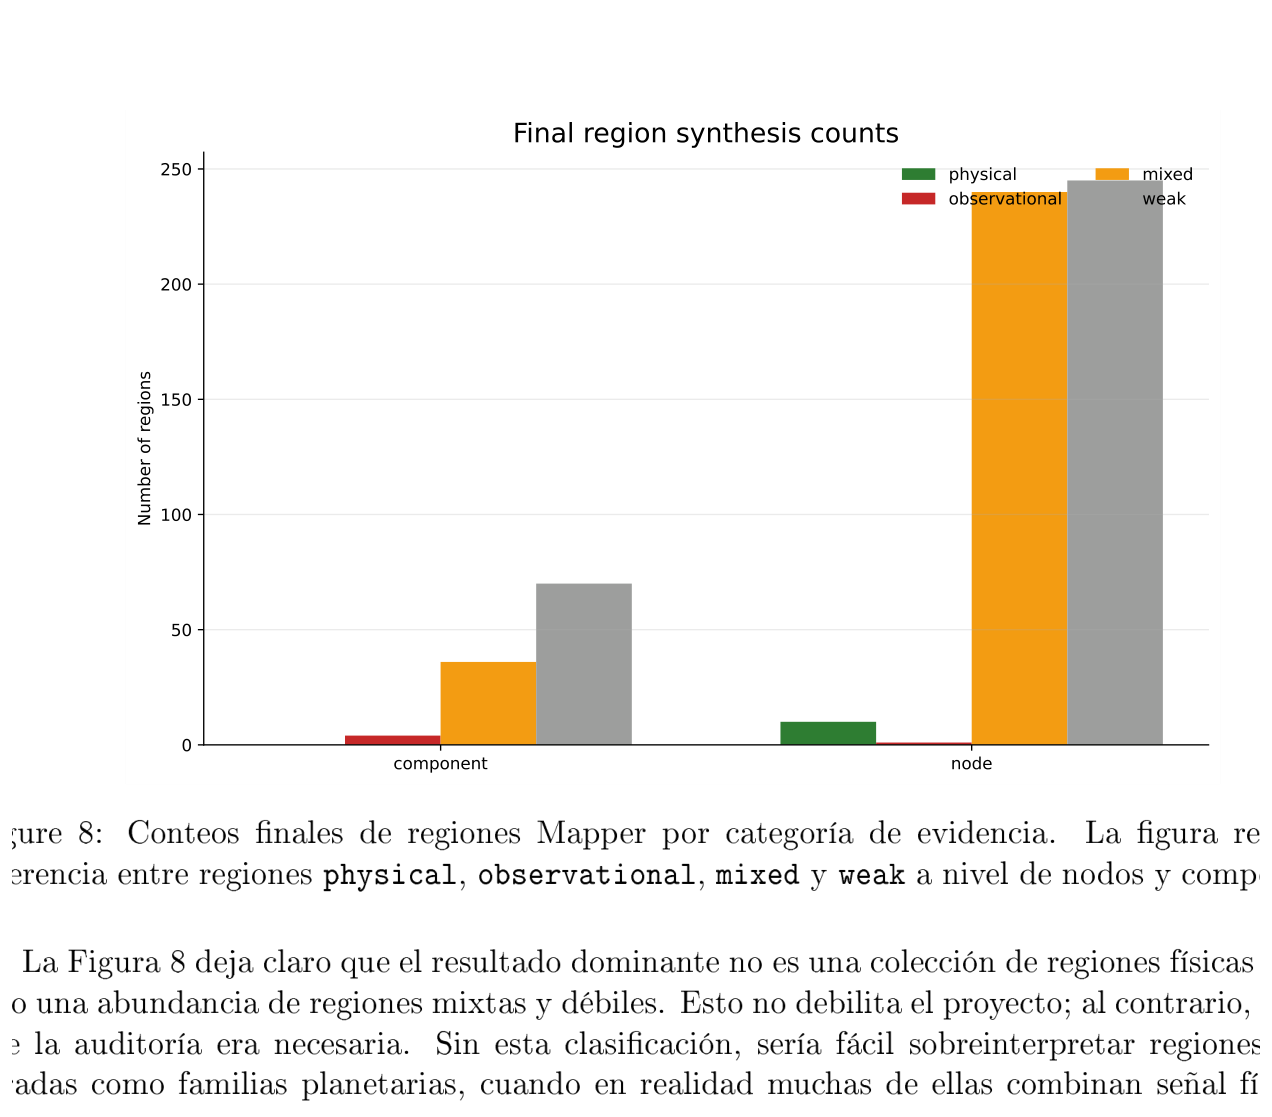
\includegraphics[width=0.75\textwidth]{fig06_final_region_synthesis_counts.png}
\caption{Conteos finales de regiones por categoría de evidencia. El predominio de regiones mixtas muestra que el catálogo combina señal física-orbital, método de descubrimiento e incertidumbre de datos.}
\end{figure}

\begin{figure}[H]
\centering
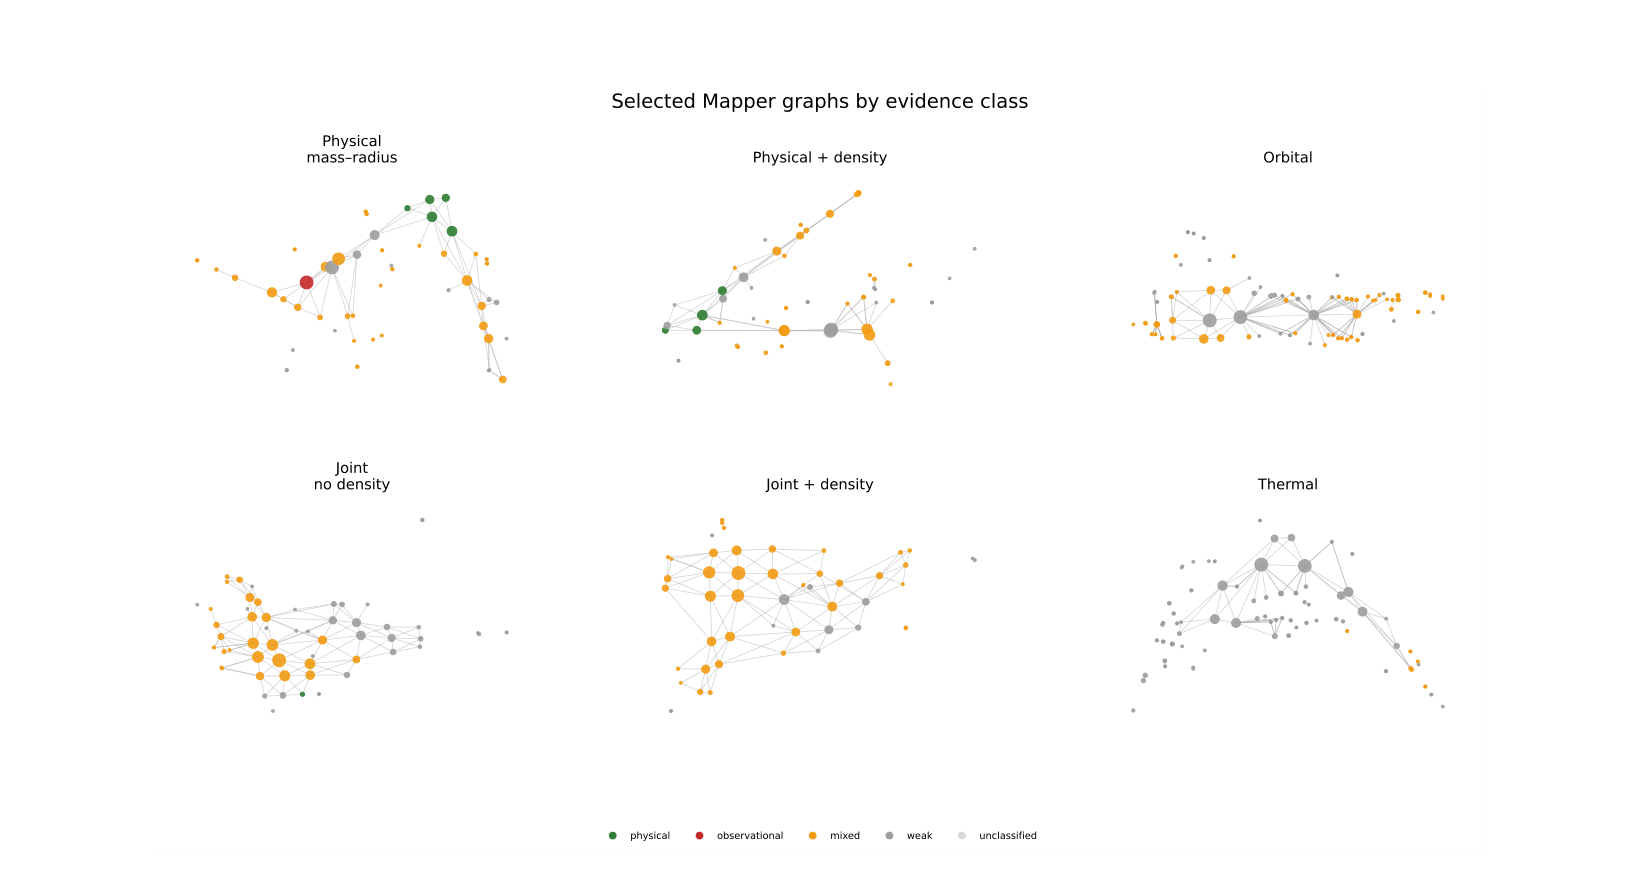
\includegraphics[width=0.98\textwidth]{fig07_selected_graphs_by_evidence.png}
\caption{Grafos seleccionados coloreados por categoría final de evidencia. Esta visualización desplaza la pregunta desde qué grafo tiene más estructura hacia qué tipo de evidencia sostiene cada región.}
\end{figure}

\executivebox{softblue}{\textbf{Síntesis.} La clasificación final mejora la interpretabilidad: permite destacar regiones con señal limpia, separar regiones dominadas por proceso observacional y mantener regiones mixtas como oportunidades de inspección más fina.}

\section{El grafo orbital: el núcleo más informativo del proyecto}

El grafo orbital concentra la narrativa científica más útil. Su complejidad indica riqueza estructural; su baja imputación lo vuelve confiable como base analítica; su asociación con método de descubrimiento lo convierte en el puente natural hacia sombra observacional y priorización.

\begin{figure}[H]
\centering
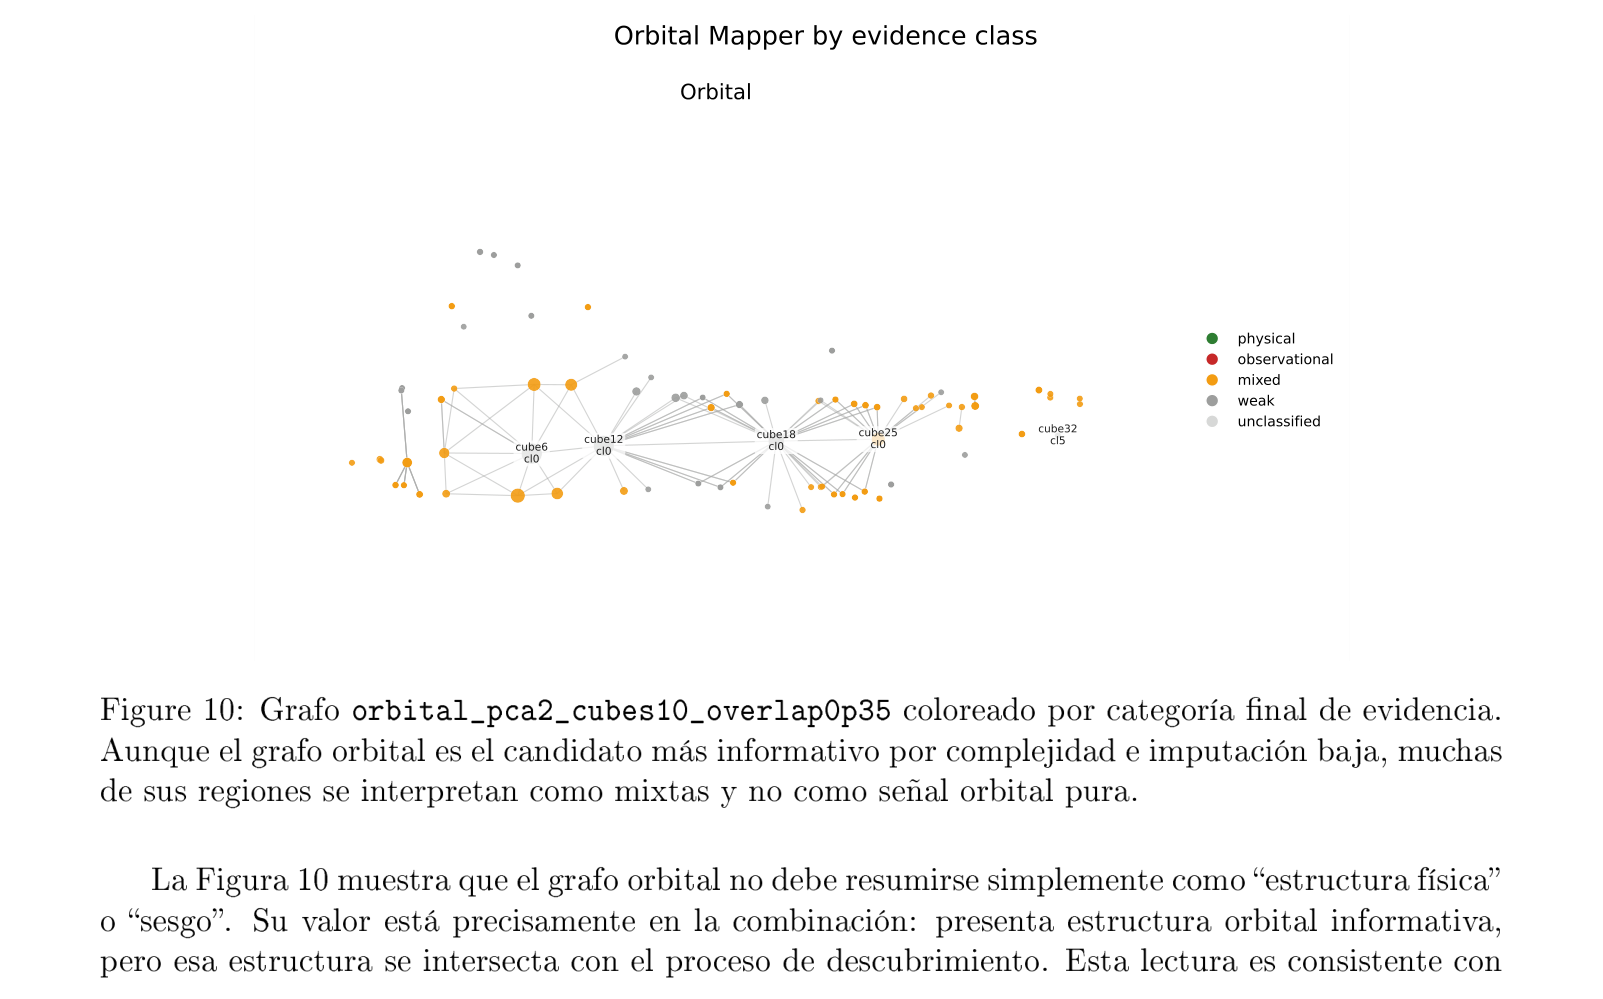
\includegraphics[width=0.9\textwidth]{fig08_orbital_mapper_evidence_class.png}
\caption{Grafo orbital coloreado por clase final de evidencia. El valor del grafo está en su mezcla: estructura orbital rica, baja imputación y regiones que requieren lectura observacional cuidadosa.}
\end{figure}

\begin{figure}[H]
\centering
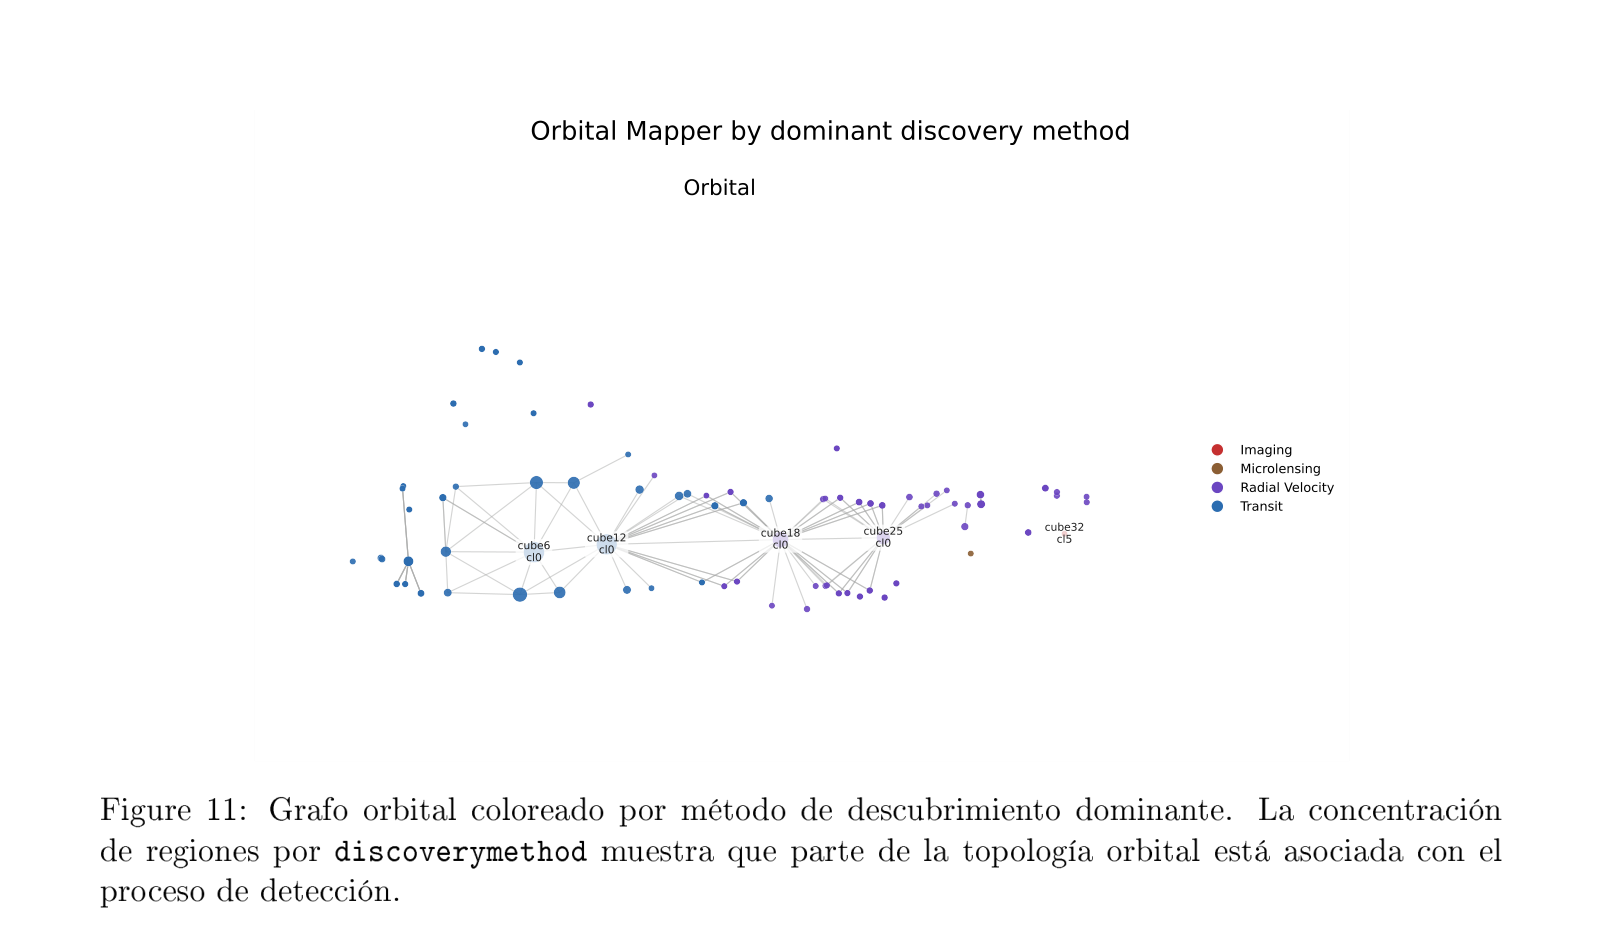
\includegraphics[width=0.9\textwidth]{fig09_orbital_mapper_method.png}
\caption{Grafo orbital coloreado por método de descubrimiento dominante. Las regiones de tránsito y velocidad radial muestran que la topología del catálogo conserva huellas del proceso de detección.}
\end{figure}

\begin{figure}[H]
\centering
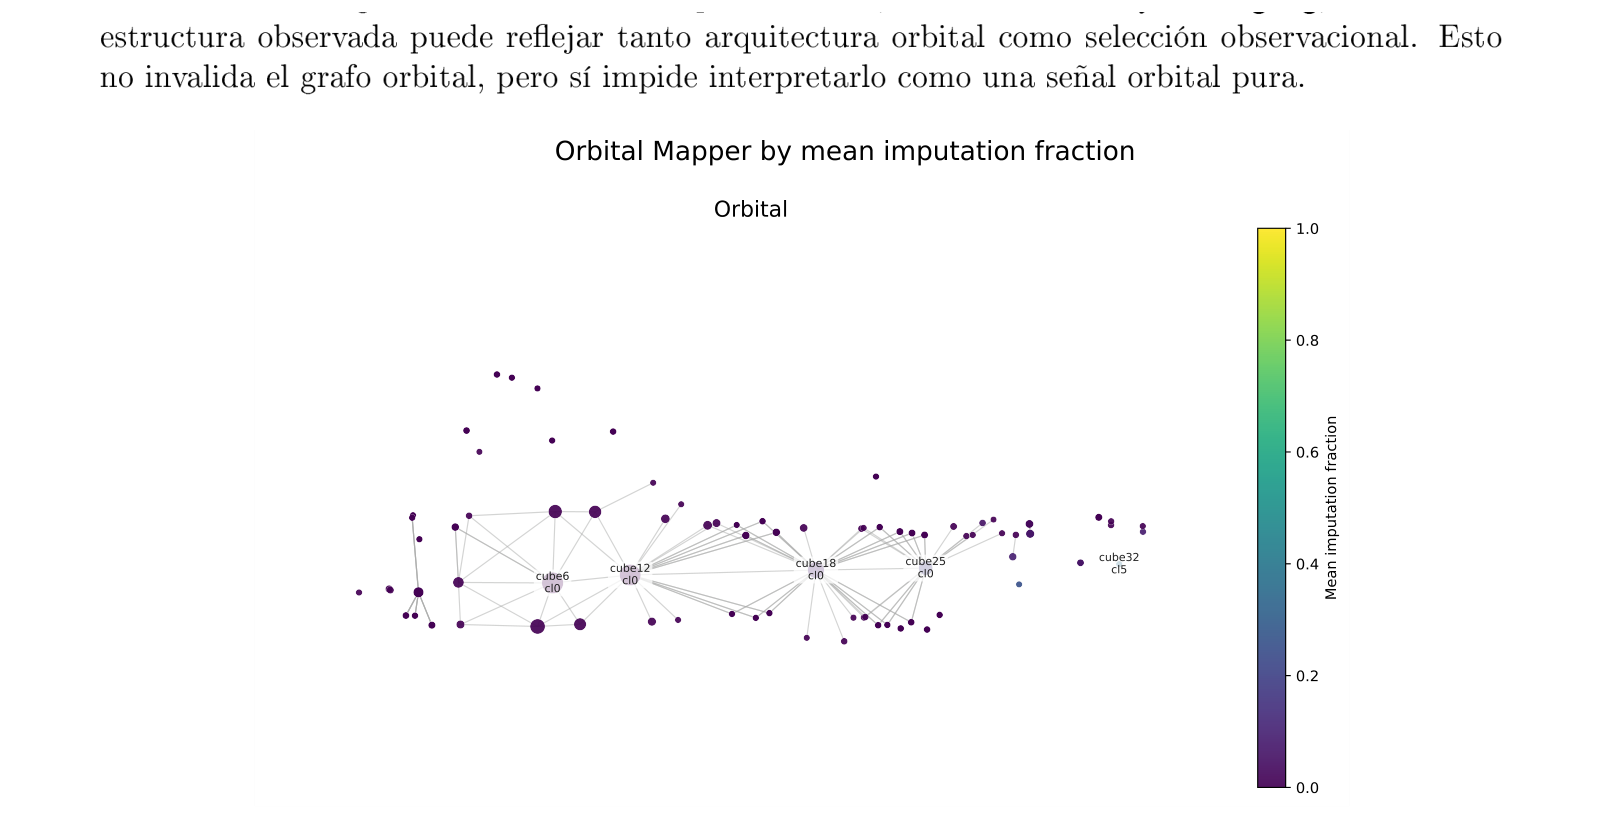
\includegraphics[width=0.9\textwidth]{fig10_orbital_mapper_imputation.png}
\caption{Grafo orbital coloreado por fracción de imputación. La baja imputación general refuerza la utilidad del espacio orbital para inspección, mientras la auditoría por método orienta la lectura hacia sesgo de descubrimiento.}
\end{figure}

Esta triple lectura es una de las mejores aportaciones del proyecto: el espacio orbital es topológicamente rico, está bien sostenido por datos y conserva señal observacional. Por eso funciona como plataforma para formular índices de sombra e incompletitud topológica.

\section{Del sesgo de descubrimiento a la sombra observacional}

La auditoría observacional mostró que los métodos de descubrimiento están organizados dentro del grafo. El siguiente paso fue convertir esa observación en un índice local: la sombra observacional. La sombra no premia simplemente que un nodo sea puro por método; premia que el nodo contraste con sus vecinos, tenga baja imputación y soporte suficiente. Con esto, el proyecto pasa de una lectura descriptiva a una lectura accionable.

\begin{center}
\fcolorbox{navy}{softgreen}{\begin{minipage}{0.86\textwidth}
\[
\begin{aligned}
&\text{método dominante}+\text{contraste con vecinos}+\text{baja imputación}+\text{soporte de red}\\
&\Rightarrow \text{región candidata a inspección}
\end{aligned}
\]
\end{minipage}}
\end{center}

En términos astronómicos, las comunidades dominadas por velocidad radial son especialmente interesantes porque su ventana de detección favorece objetos con señal dinámica suficiente. Una región RV de alta sombra puede sugerir vecindades donde el catálogo tiene mayor información esperada hacia masas menores, señales radiales más débiles o mejores mediciones futuras.

\section{TOI: prioridad regional}

TOI formaliza la lectura regional. Un nodo sube en el ranking si combina sombra observacional, baja imputación en \(R^3\), continuidad física con vecinos y soporte de red. Esta combinación es importante: transforma sesgo en prioridad solo cuando la señal aparece en una región físicamente auditable.

\[
\mathrm{TOI}(v)=\mathrm{Shadow}(v)\,(1-I_{R^3}(v))\,C_{\mathrm{phys}}(v)\,S_{\mathrm{net}}(v).
\]

\begin{figure}[H]
\centering
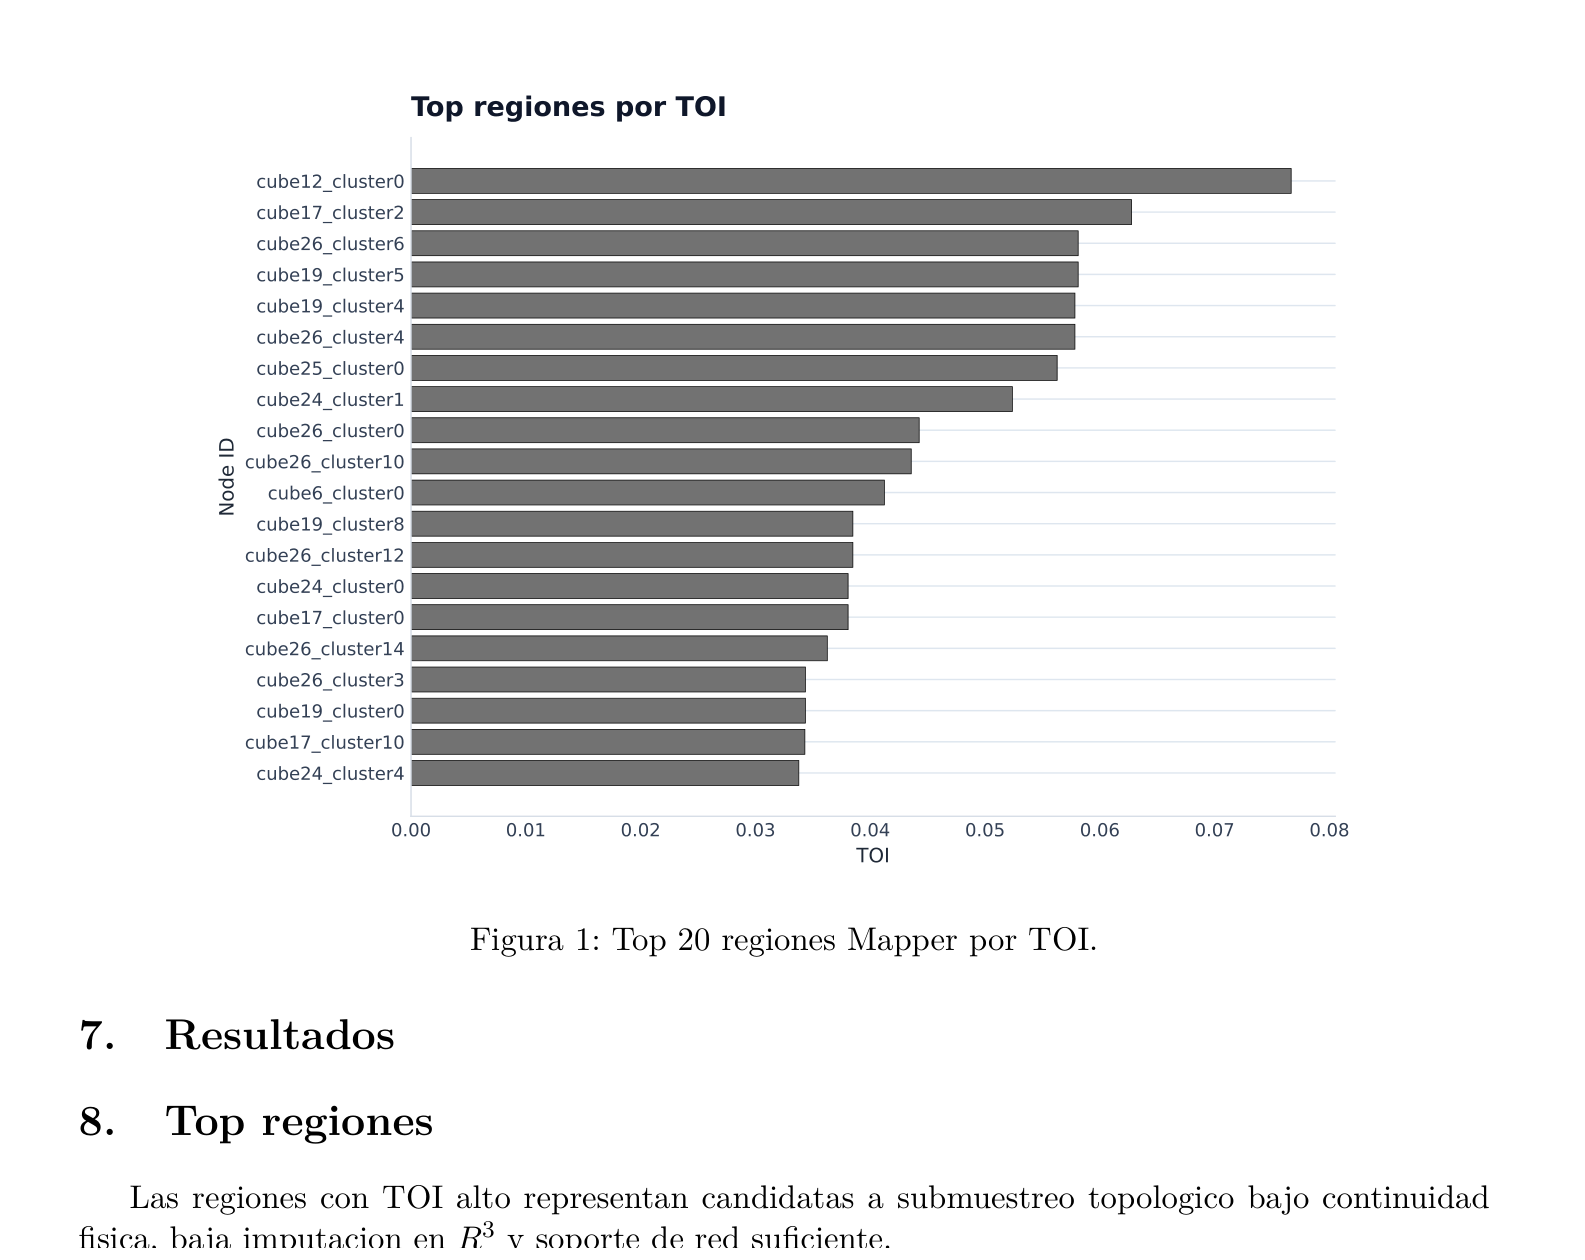
\includegraphics[width=0.85\textwidth]{fig11_top_regions_toi.png}
\caption{Top regiones por TOI. \code{cube12\_cluster0} aparece como la región regionalmente más prioritaria, seguida por \code{cube17\_cluster2} y nodos cercanos en el ranking.}
\end{figure}

\begin{figure}[H]
\centering
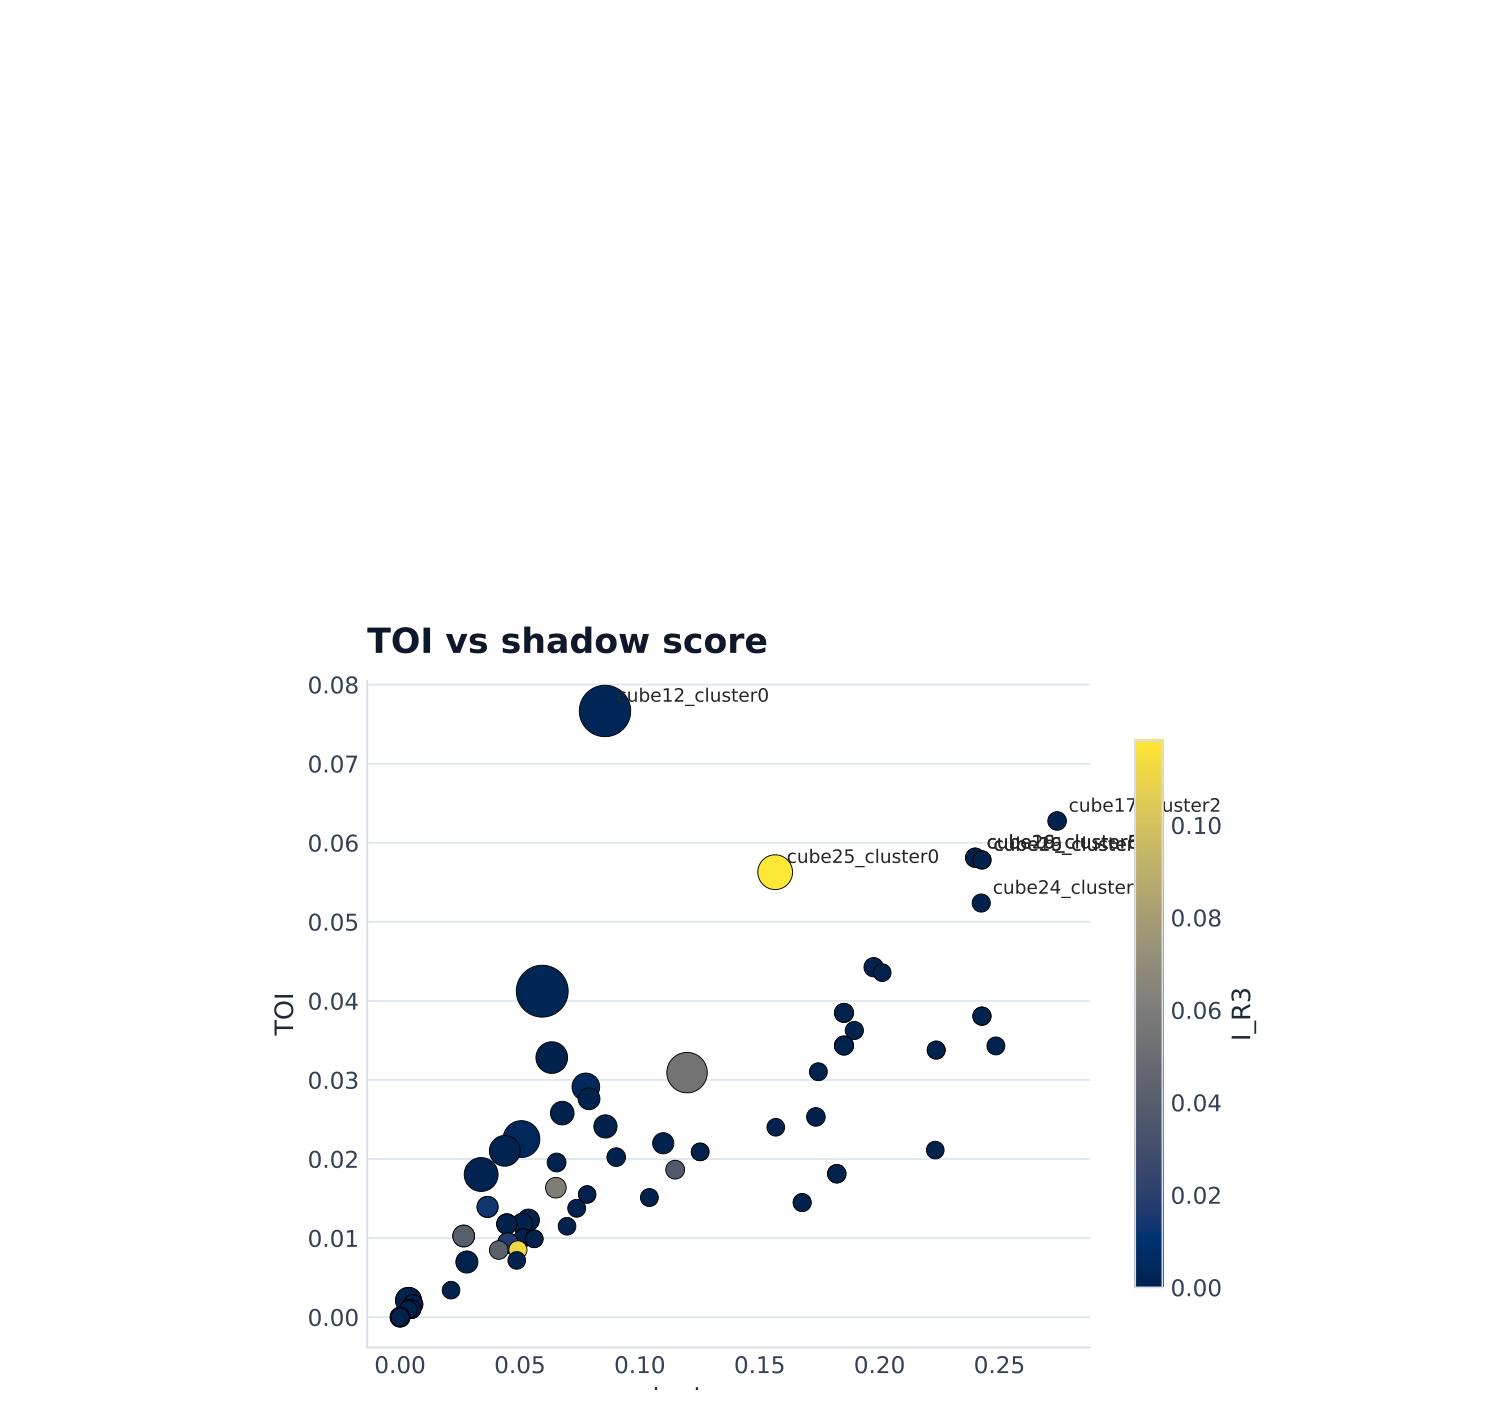
\includegraphics[width=0.82\textwidth]{fig13_toi_vs_shadow.png}
\caption{Relación entre sombra observacional y TOI. El resultado muestra que TOI no replica mecánicamente la sombra: agrega trazabilidad, continuidad física y soporte topológico.}
\end{figure}

\executivebox{softorange}{\textbf{Resultado regional.} \code{cube12\_cluster0} es la mejor región para explicar el índice TOI: combina sombra observacional, baja dependencia de imputación, continuidad física y soporte de red.}

\section{ATI: de regiones a planetas ancla}

ATI traduce una región prioritaria en planetas ancla concretos. El ancla permite contar vecinos observados y compararlos con referencias locales en el espacio \(R^3\). La utilidad de ATI es comunicacional y operativa: convierte un nodo Mapper en una ficha de inspección.

\[
\mathrm{ATI}(p^*)=\mathrm{TOI}(v)\,\Delta_{\mathrm{rel,best}}(p^*)\,(1-I_{R^3}(p^*))\,A(p^*),\qquad p^*\in S_v.
\]

\begin{figure}[H]
\centering
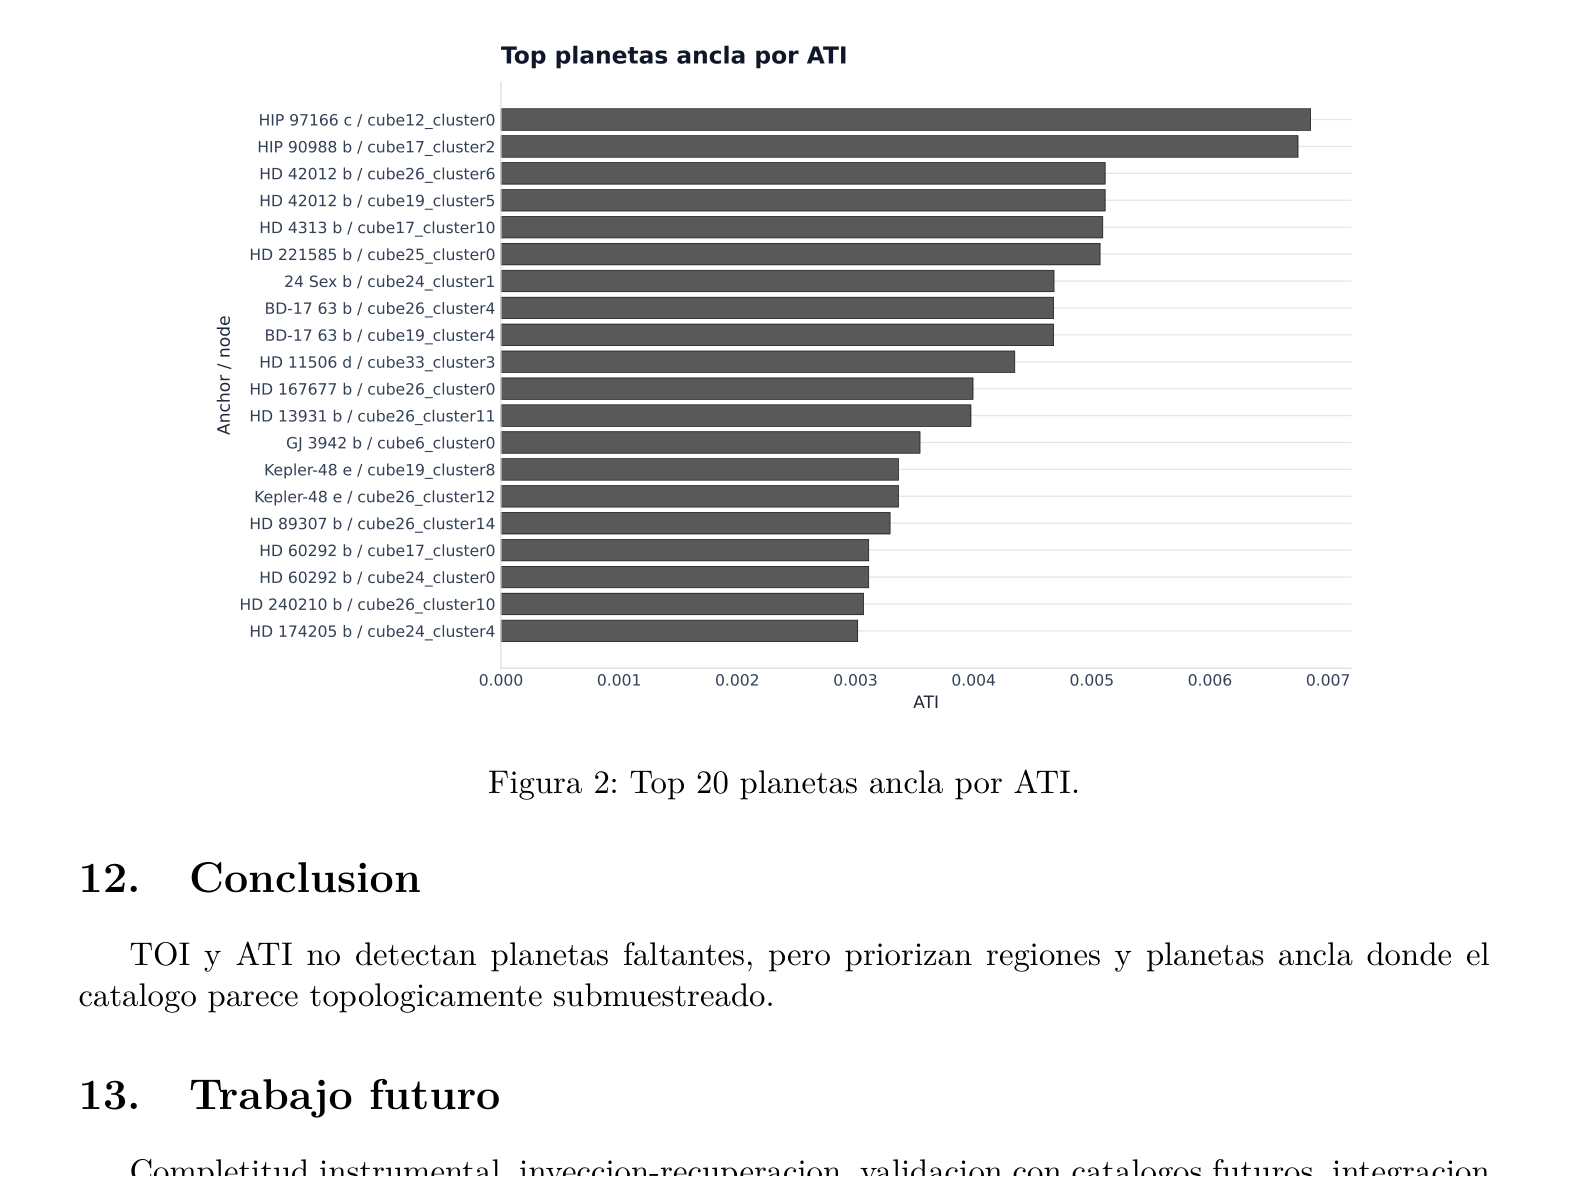
\includegraphics[width=0.85\textwidth]{fig12_top_anchors_ati.png}
\caption{Top planetas ancla por ATI original. HIP 97166 c aparece como ancla exploratoria principal; HIP 90988 b queda inmediatamente como caso fuerte para validación conservadora.}
\end{figure}

El índice ATI original fue exitoso como detector exploratorio: encontró anclas locales destacadas. La validación final refinó la narrativa al preguntar si el déficit se mantiene cuando cambia la escala del radio. Ese ajuste convirtió un ranking prometedor en un ranking más defendible para exposición y trabajo futuro.

\section{Validación multiescala: del ranking exploratorio al ranking conservador}

El paso metodológico más importante de la fase final fue separar señales exploratorias de prioridades conservadoras. El término \(\Delta_{\mathrm{rel,best}}\) toma el radio más favorable; eso es útil para descubrir candidatos, pero la exposición final favorece anclas cuyo déficit se mantiene positivo al evaluar \(r_{\mathrm{kNN}}\), \(r_{\mathrm{node\_median}}\) y \(r_{\mathrm{node\_q75}}\).

\begin{figure}[H]
\centering
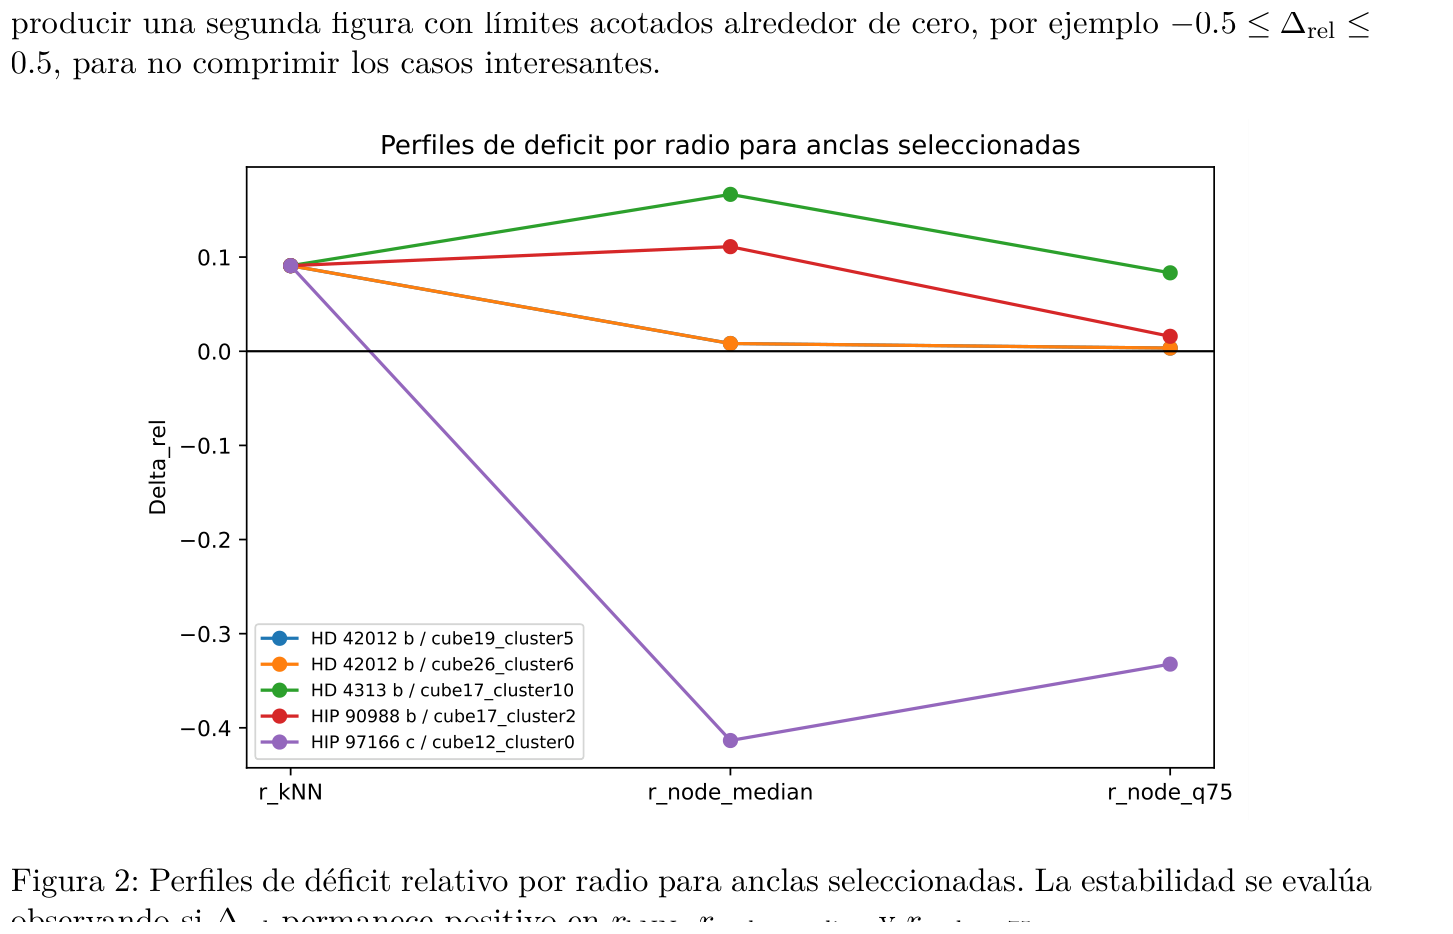
\includegraphics[width=0.82\textwidth]{fig14_deficit_profiles_by_radius.png}
\caption{Perfiles de déficit relativo por radio. HIP 97166 c ilustra sensibilidad a escala; HIP 90988 b conserva una señal positiva en las tres escalas evaluadas.}
\end{figure}

\begin{figure}[H]
\centering
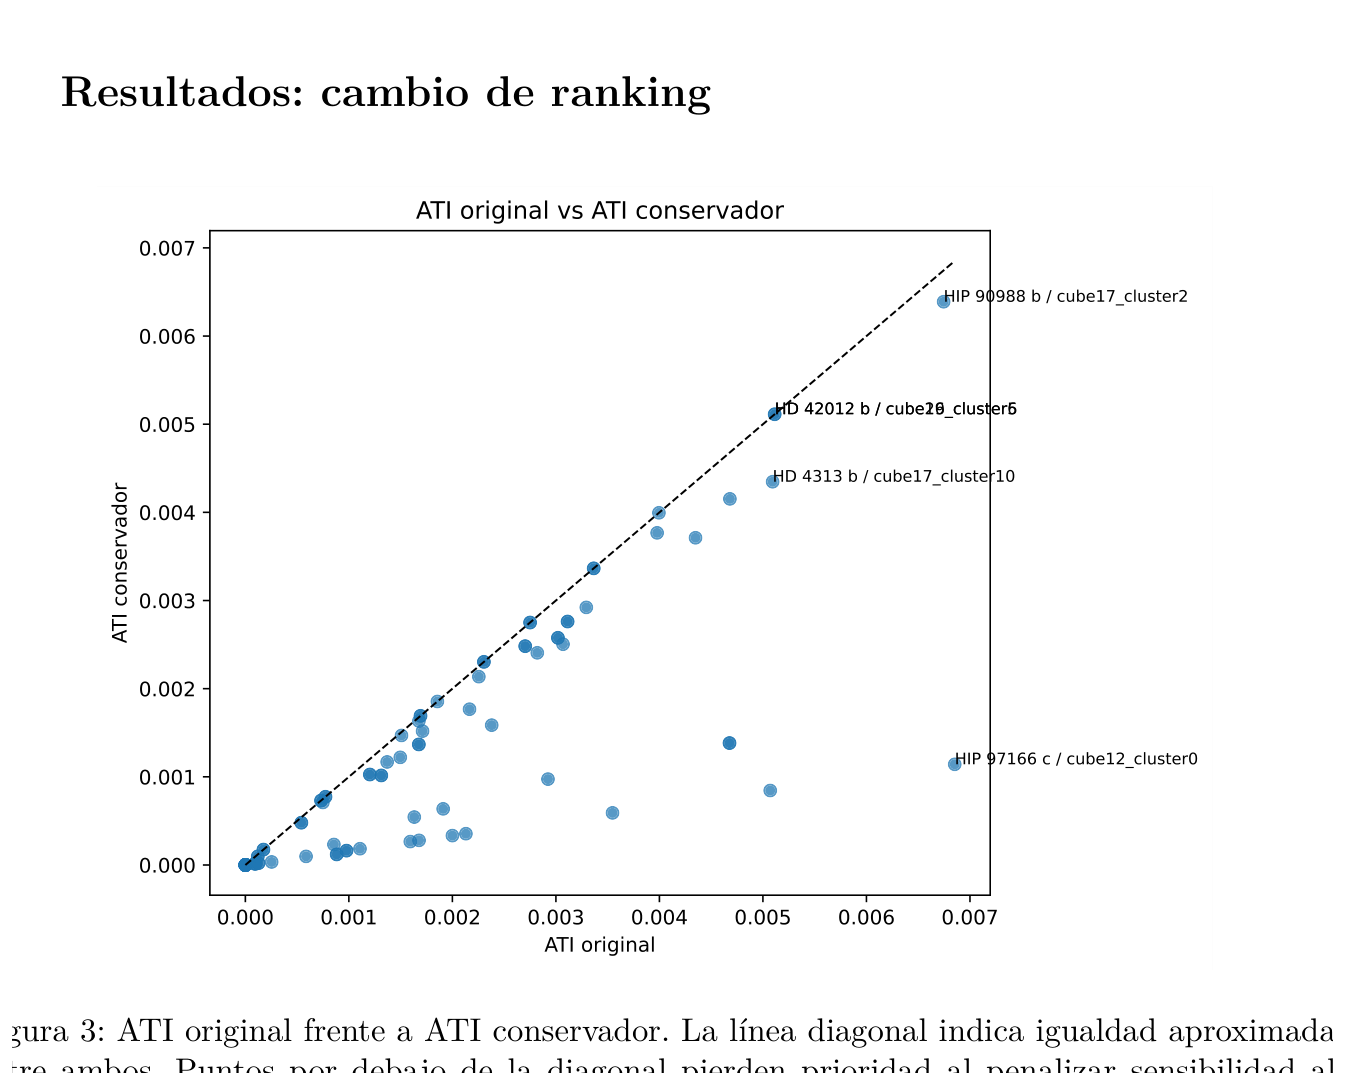
\includegraphics[width=0.78\textwidth]{fig15_ati_original_vs_conservative.png}
\caption{ATI original frente a ATI conservador. La penalización multiescala desplaza la narrativa final hacia casos más estables, especialmente HIP 90988 b.}
\end{figure}

\executivebox{softgreen}{\textbf{Resultado conservador.} HIP 90988 b / \code{cube17\_cluster2} emerge como la ancla final más defendible: su déficit es pequeño, pero estable, y su región conserva TOI alto con lectura RV coherente.}

\section{Ranking final de prioridad observacional}

La lectura final se expresa como ranking de prioridad observacional. El ranking ordena anclas donde nuevas observaciones, mejores mediciones o modelos de completitud podrían aportar más información bajo la referencia topológica local.

\begin{figure}[H]
\centering
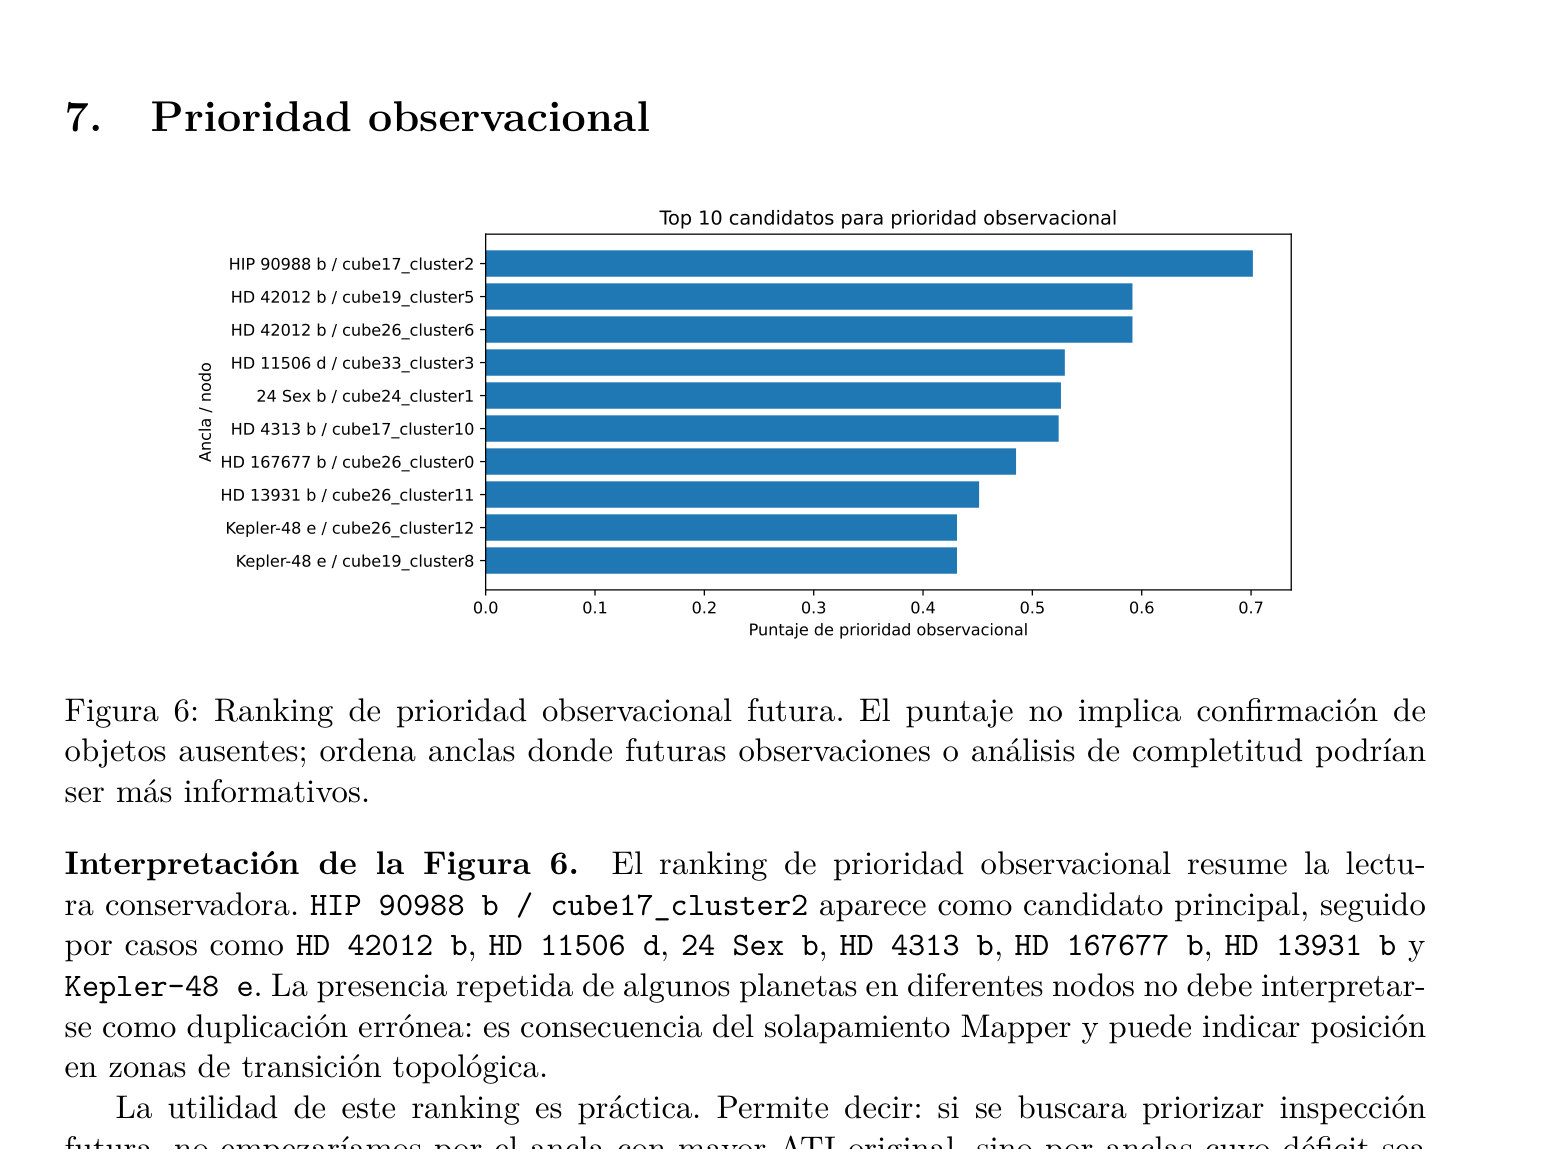
\includegraphics[width=0.86\textwidth]{fig16_observational_priority_ranking.png}
\caption{Top 10 candidatos de prioridad observacional. HIP 90988 b / \code{cube17\_cluster2} encabeza la lista conservadora; HD 42012 b aparece como ancla de transición en más de un nodo.}
\end{figure}

\begin{center}
\small
\begin{tabular}{@{}cll@{}}
\toprule
\textbf{Rank} & \textbf{Ancla} & \textbf{Nodo} \\
\midrule
1 & HIP 90988 b & \code{cube17\_cluster2} \\
2 & HD 42012 b & \code{cube19\_cluster5} \\
3 & HD 42012 b & \code{cube26\_cluster6} \\
4 & HD 11506 d & \code{cube33\_cluster3} \\
5 & 24 Sex b & \code{cube24\_cluster1} \\
6 & HD 4313 b & \code{cube17\_cluster10} \\
7 & HD 167677 b & \code{cube26\_cluster0} \\
8 & HD 13931 b & \code{cube26\_cluster11} \\
9 & Kepler-48 e & \code{cube26\_cluster12} \\
10 & Kepler-48 e & \code{cube19\_cluster8} \\
\bottomrule
\end{tabular}
\end{center}

\section{Fichas finales: los casos que cuentan la historia}

La exposición final queda más clara al usar cuatro tipos de casos: una región top, una ancla conservadora, una ancla de transición y un candidato secundario estable.

\begin{figure}[H]
\centering
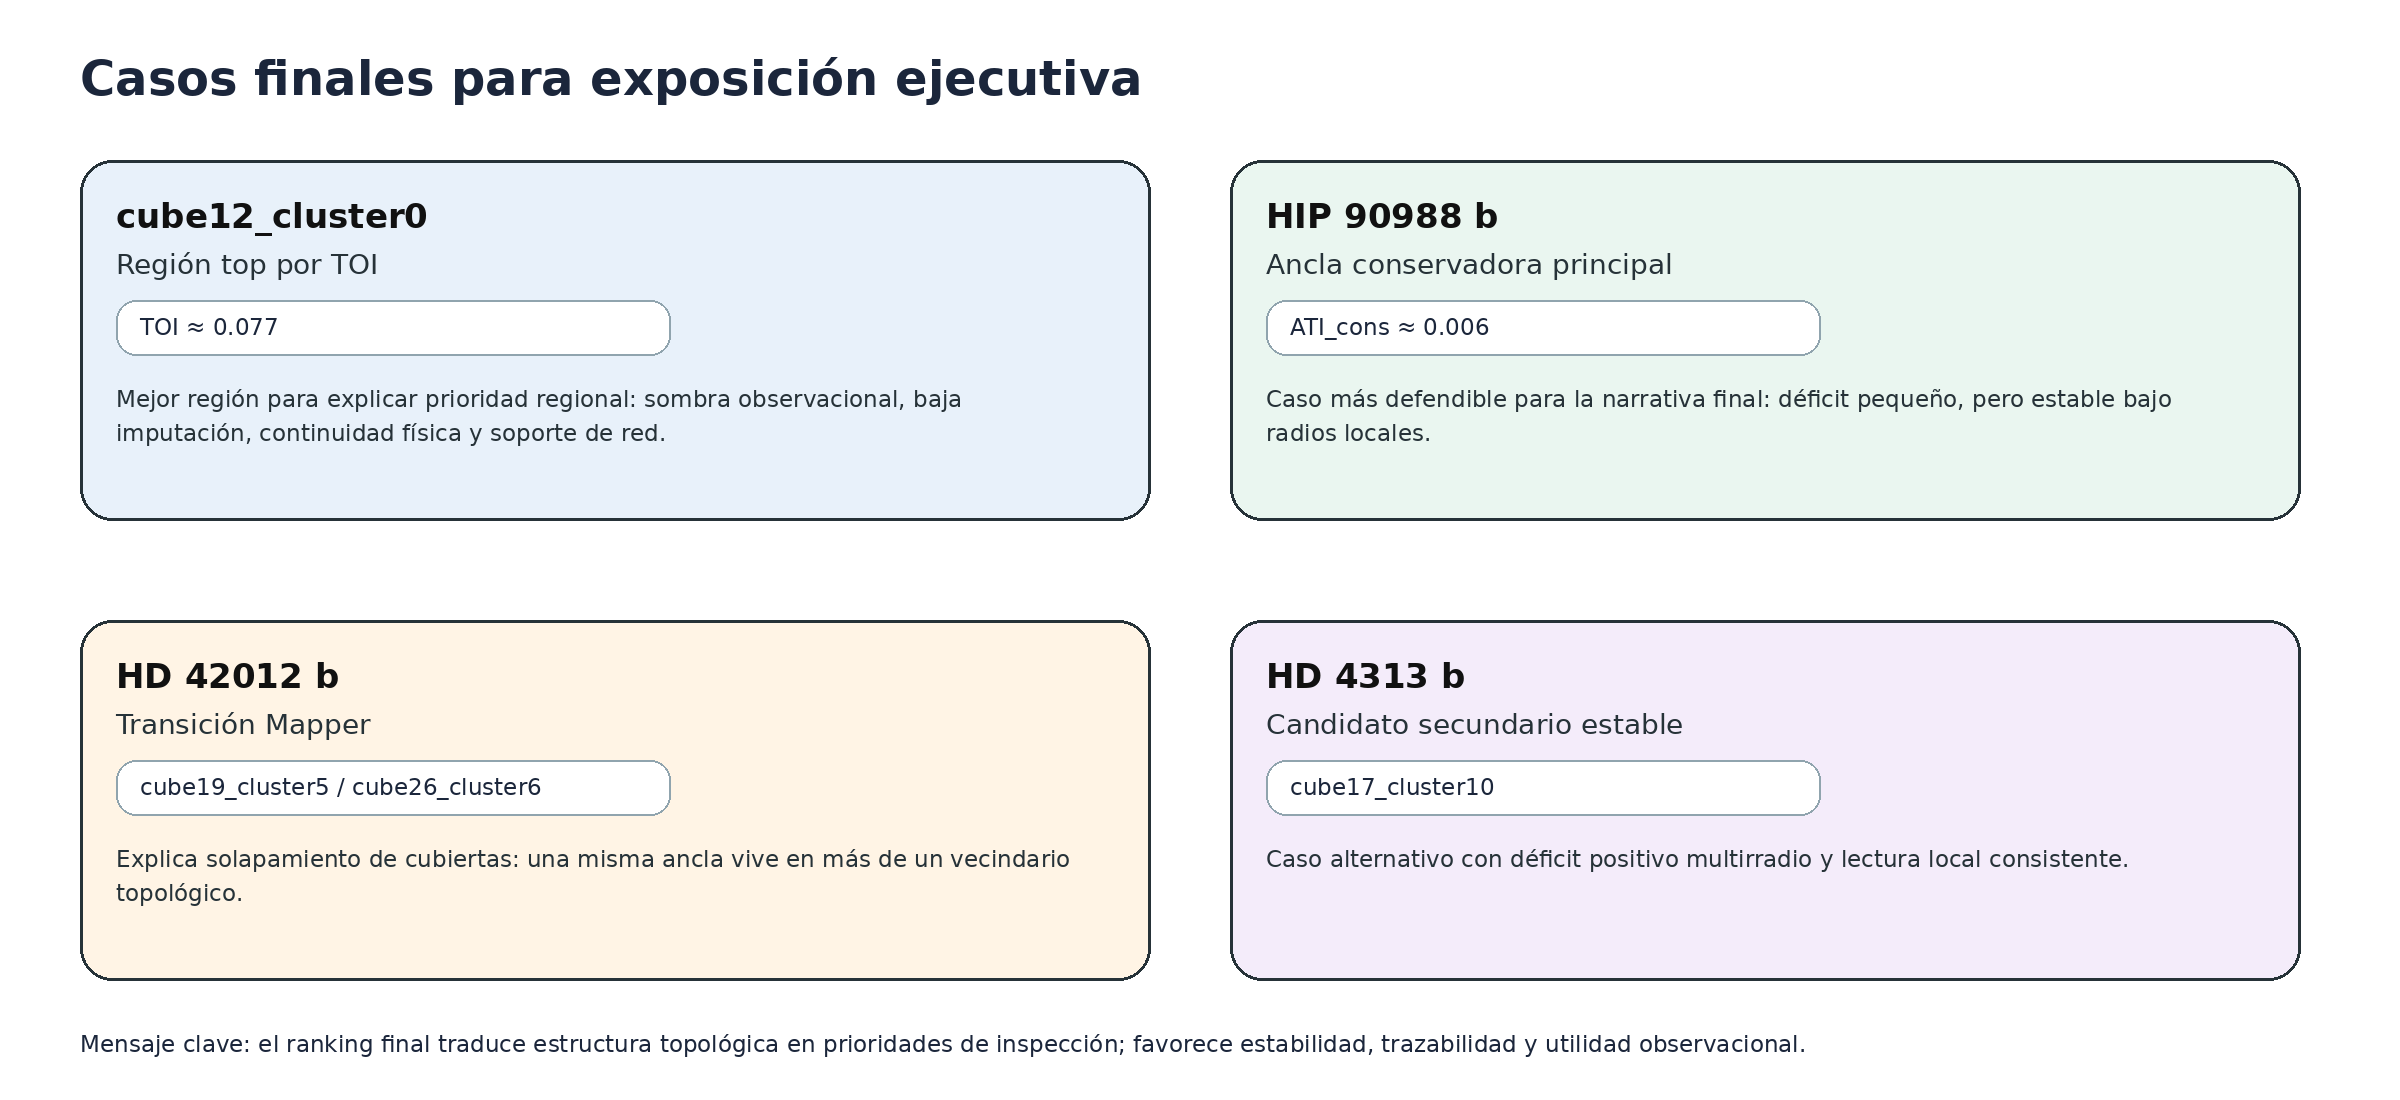
\includegraphics[width=0.98\textwidth]{fig23_final_case_cards.png}
\caption{Casos finales recomendados para exposición ejecutiva. La selección comunica la historia completa: región regional, ancla robusta, transición Mapper y soporte secundario estable.}
\end{figure}

\subsection{Región top por TOI: \code{cube12\_cluster0}}

\code{cube12\_cluster0} concentra la mejor lectura regional del pipeline. Su valor aproximado \(\mathrm{TOI}\approx 0.077\) resume una combinación de sombra observacional, baja imputación, continuidad física y soporte de red. Es el punto más directo para explicar qué significa convertir sesgo en prioridad regional.

\subsection{Ancla conservadora: HIP 90988 b / \code{cube17\_cluster2}}

HIP 90988 b es el caso final más defendible bajo ATI conservador. El nodo \code{cube17\_cluster2} está dominado por velocidad radial, tiene sombra alta, frontera metodológica fuerte, imputación nula en las variables de \(R^3\) y déficit positivo pequeño pero estable. La lectura ejecutiva es que HIP 90988 b representa una vecindad RV donde la inspección futura puede aportar información valiosa hacia objetos de menor masa o menor proxy dinámico.

\begin{figure}[H]
\centering
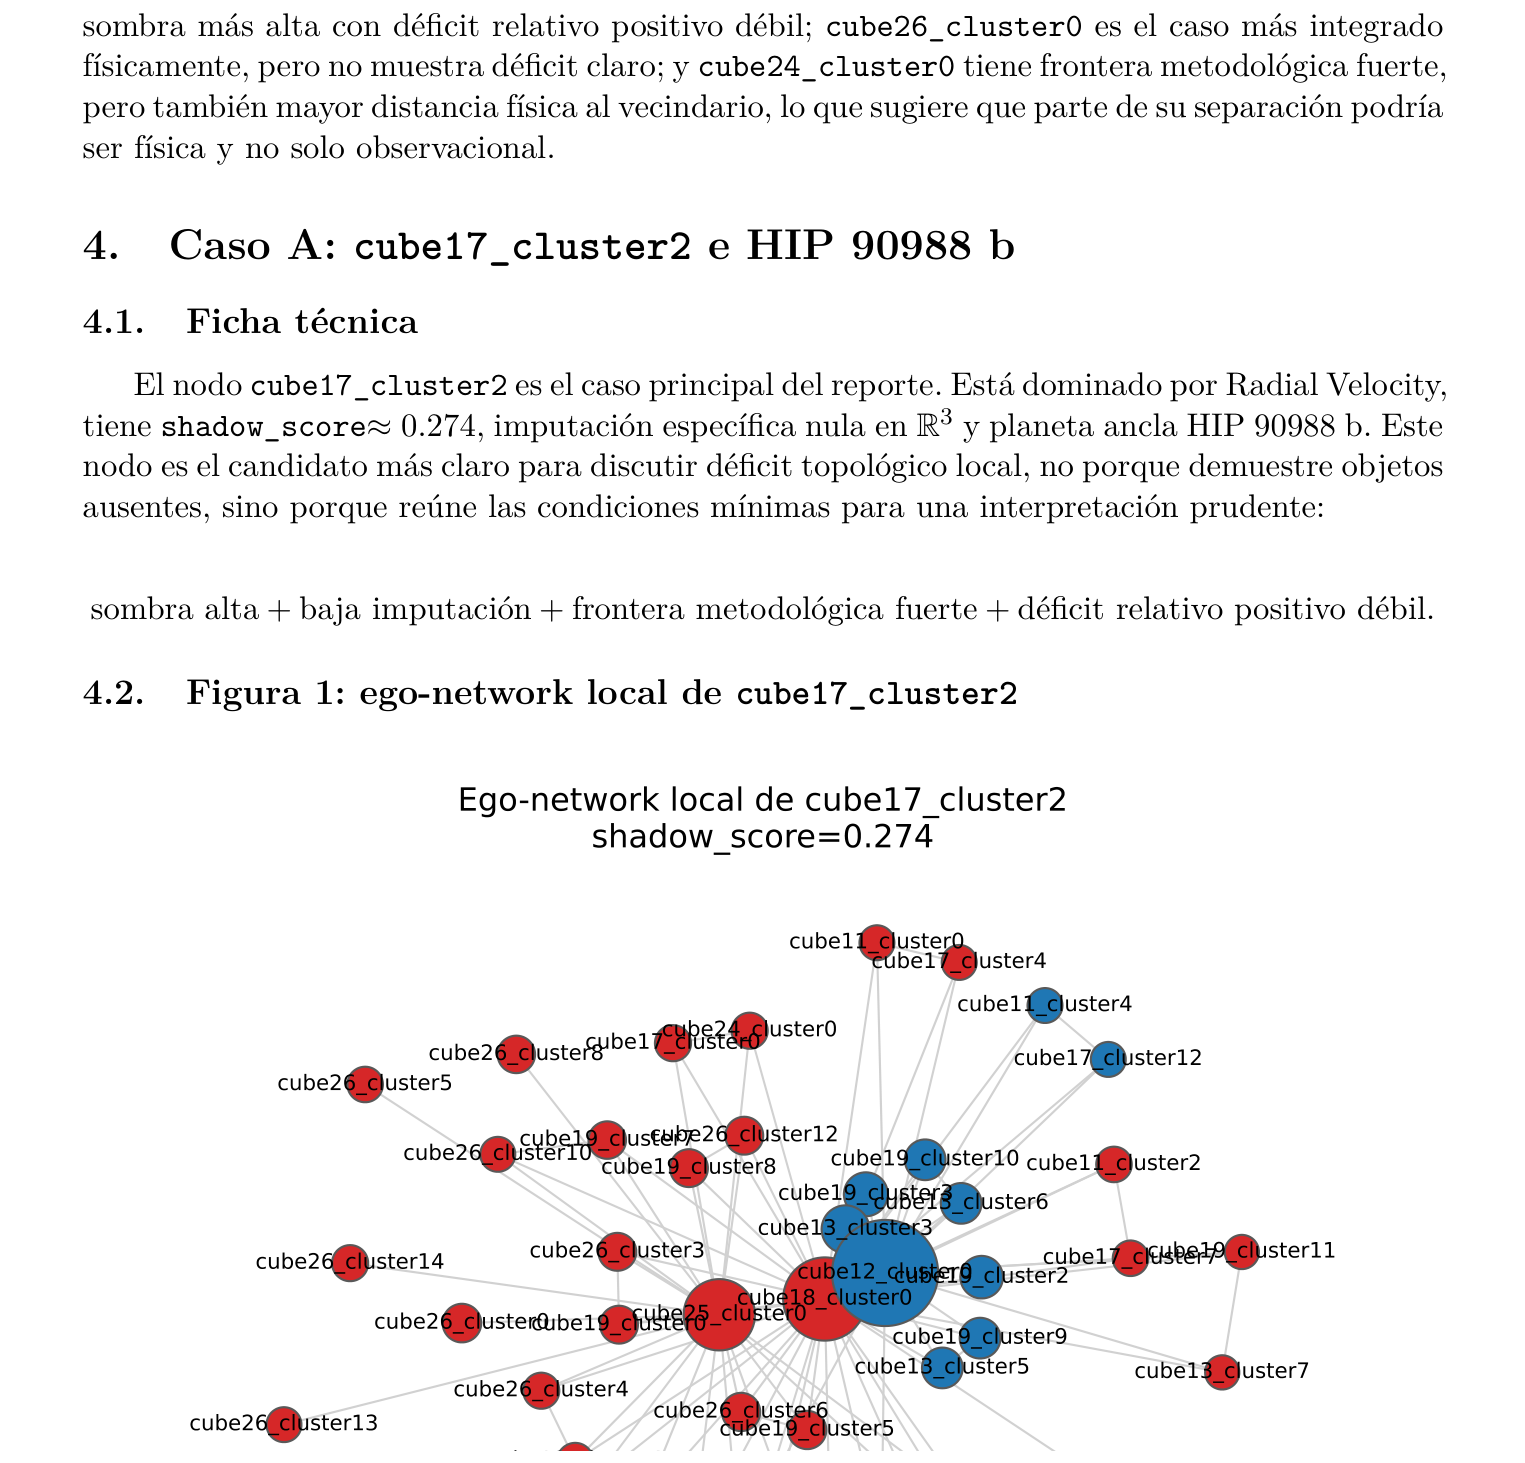
\includegraphics[width=0.82\textwidth]{fig17_hip90988_ego_network.png}
\caption{Ego-network local de \code{cube17\_cluster2}. El nodo aparece integrado en una región conectada, lo que permite comparar su composición con vecindarios de primer y segundo orden.}
\end{figure}

\begin{figure}[H]
\centering
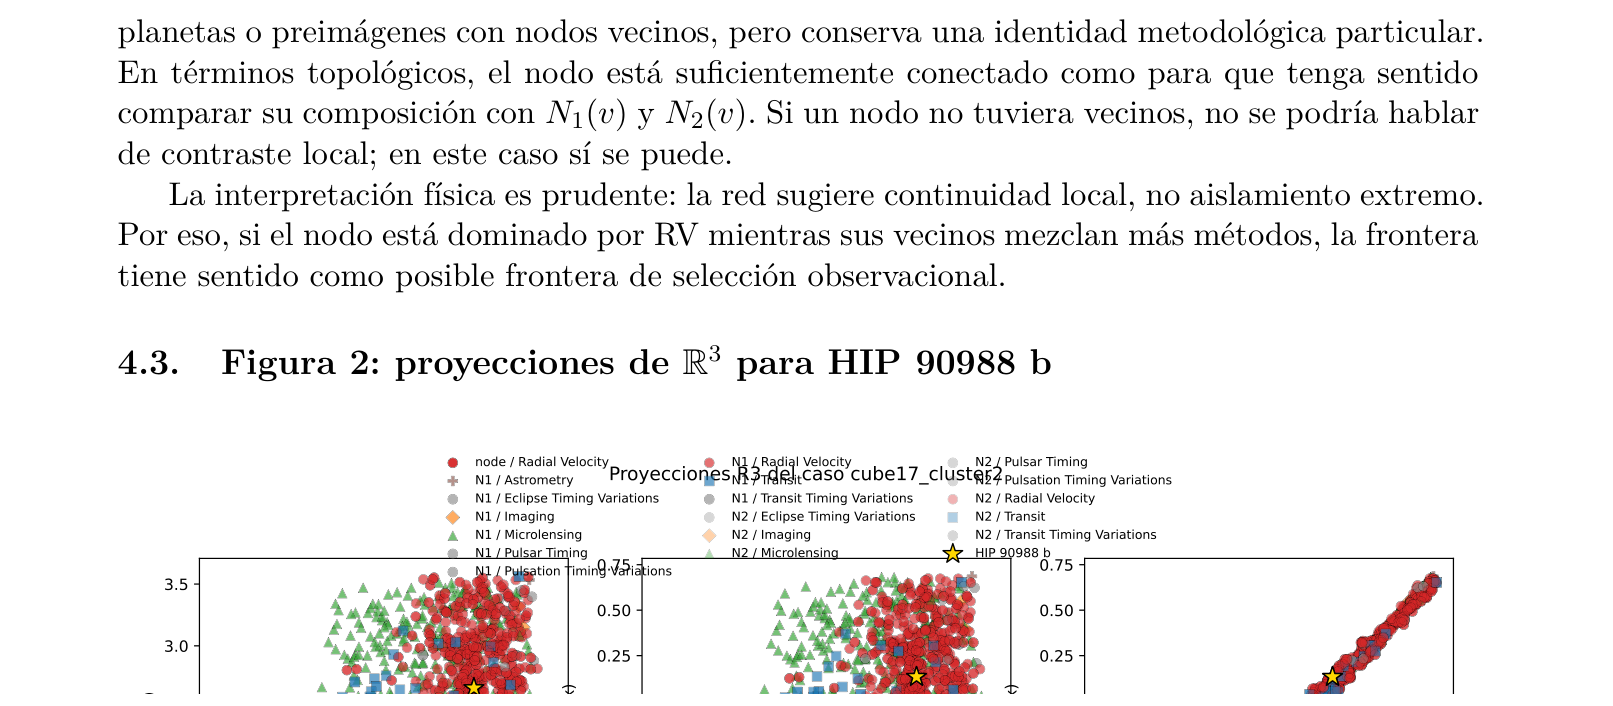
\includegraphics[width=0.95\textwidth]{fig18_hip90988_r3_projections.png}
\caption{Proyecciones de \(R^3=(\log M_p,\log P,\log a)\) para HIP 90988 b. La ancla aparece como representante local dentro de una comunidad RV, no como un objeto aislado extremo.}
\end{figure}

\begin{figure}[H]
\centering
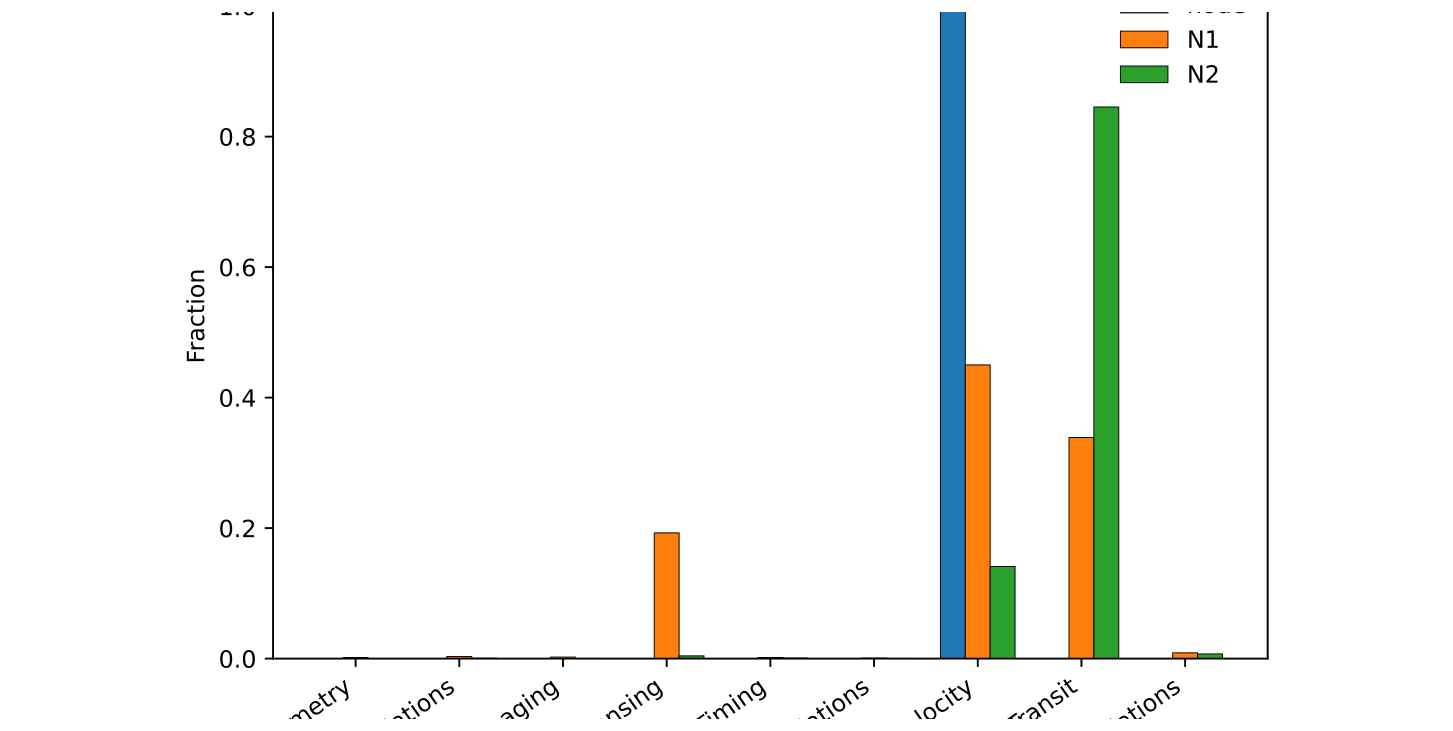
\includegraphics[width=0.84\textwidth]{fig19_hip90988_method_composition.png}
\caption{Composición por método en \code{cube17\_cluster2} y sus vecindarios. El contraste entre nodo y vecinos sostiene la lectura de frontera observacional local.}
\end{figure}

\begin{figure}[H]
\centering
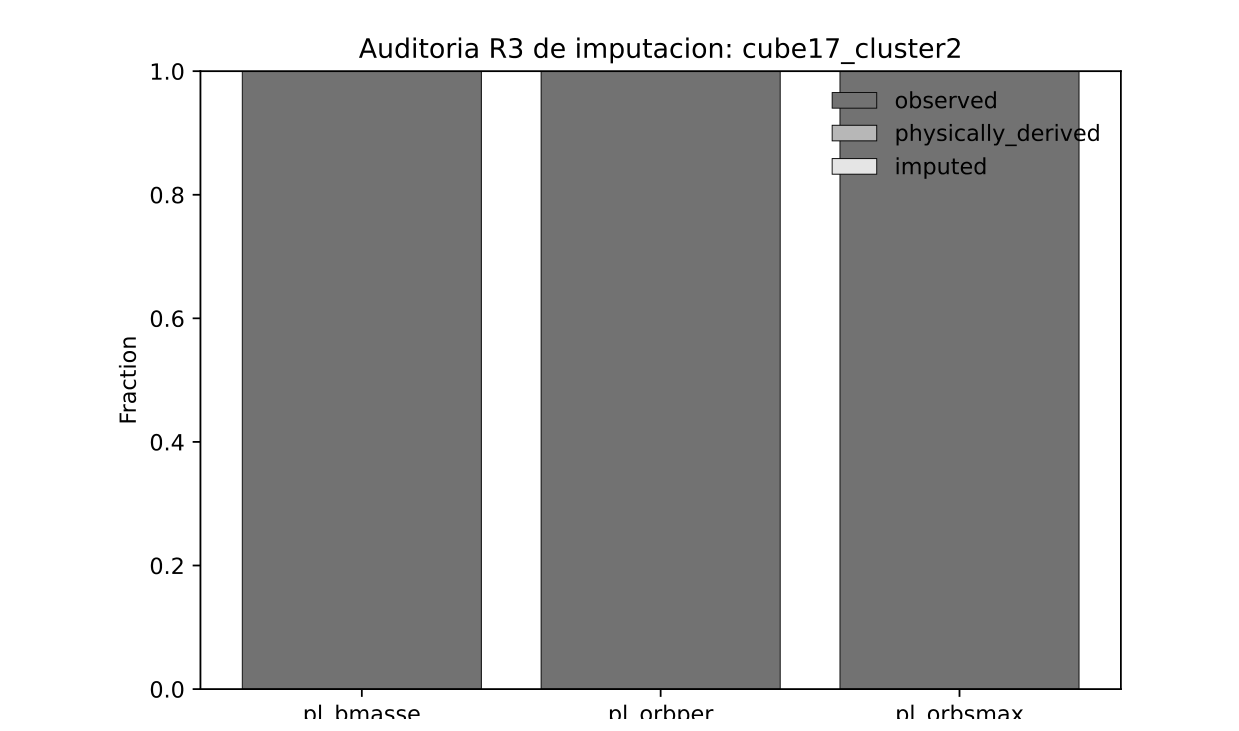
\includegraphics[width=0.78\textwidth]{fig20_hip90988_r3_audit.png}
\caption{Auditoría de imputación en \(R^3\) para \code{cube17\_cluster2}. La lectura local de masa, periodo y semieje mayor se apoya en variables disponibles para este caso.}
\end{figure}

\begin{figure}[H]
\centering
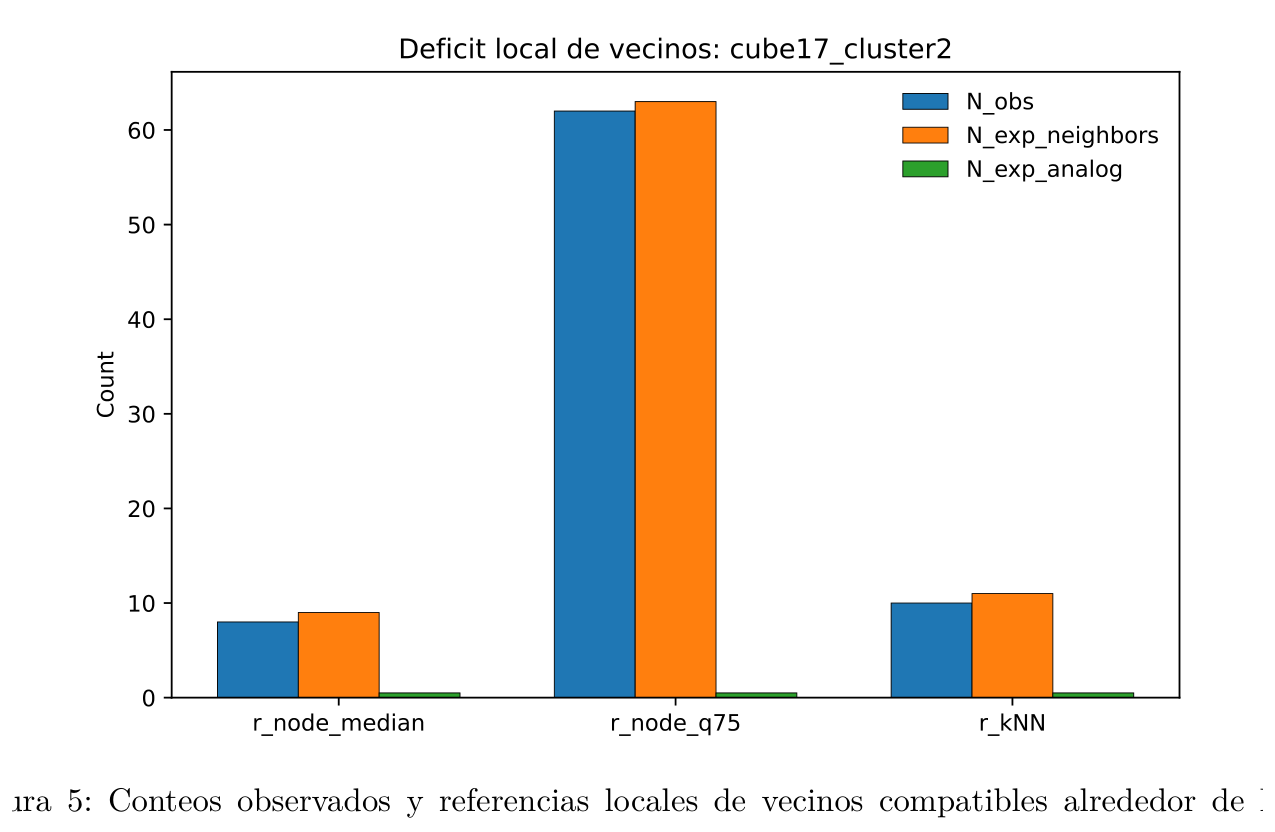
\includegraphics[width=0.78\textwidth]{fig21_hip90988_local_deficit.png}
\caption{Déficit local de vecinos compatibles alrededor de HIP 90988 b. El patrón es pequeño en magnitud, pero positivo bajo los radios evaluados.}
\end{figure}

\begin{figure}[H]
\centering
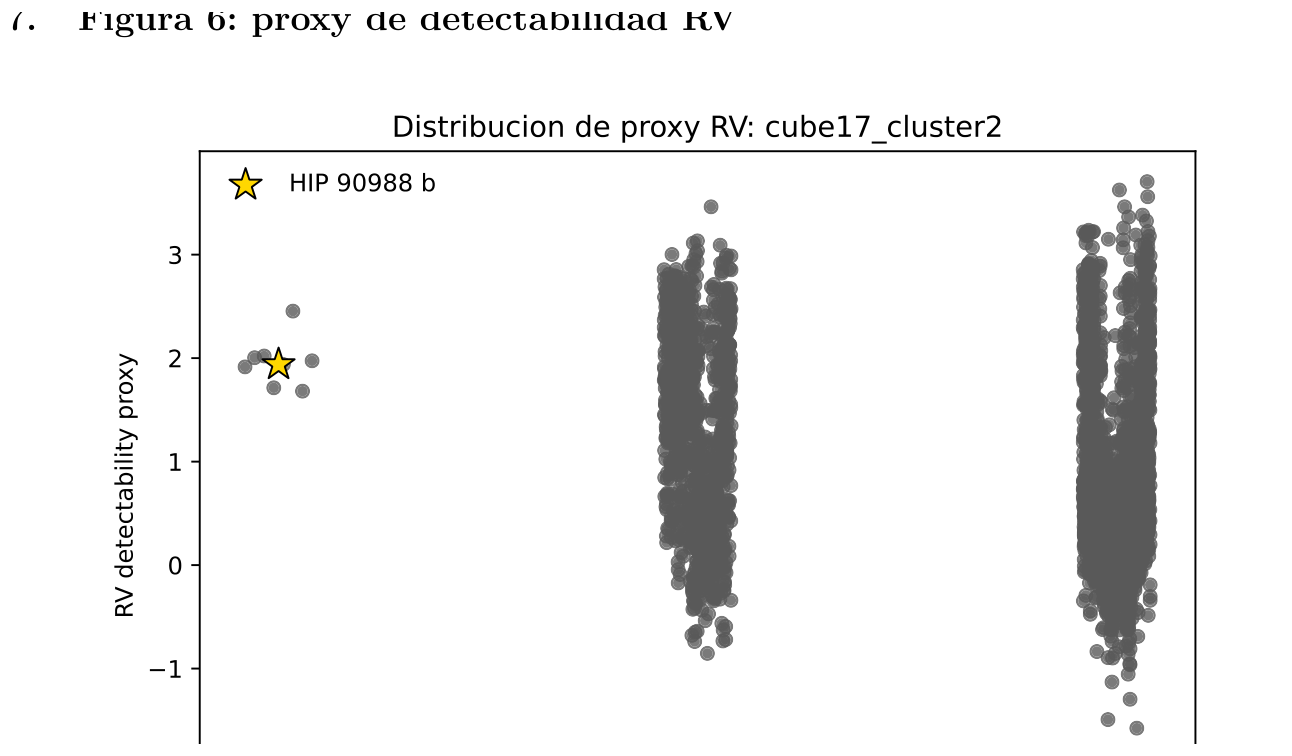
\includegraphics[width=0.78\textwidth]{fig22_hip90988_rv_proxy.png}
\caption{Proxy de detectabilidad RV para HIP 90988 b. La ancla se ubica en una región compatible con señal dinámica favorable, conectando la topología local con una lectura observacional plausible.}
\end{figure}

\subsection{Ancla de transición: HD 42012 b}

HD 42012 b aparece en \code{cube19\_cluster5} y \code{cube26\_cluster6}. Esta repetición es una propiedad esperada de Mapper: la cubierta se solapa y un mismo planeta puede vivir en más de un nodo. Su valor narrativo está en mostrar transiciones entre vecindarios físico-orbitales. En la exposición final conviene presentarlo como ejemplo de frontera topológica, no como caso de déficit fuerte.

\subsection{Candidato secundario estable: HD 4313 b}

HD 4313 b / \code{cube17\_cluster10} funciona como soporte secundario porque muestra déficit positivo más estable que HIP 97166 c. Es útil si se requiere un segundo ejemplo de ancla con señal multirradio clara, manteniendo la narrativa principal centrada en HIP 90988 b.

\section{Tesis, contrapeso y síntesis}

\textbf{Tesis.} Mapper reveló estructura relevante en el catálogo, especialmente en el espacio orbital. Esa estructura permitió construir un atlas de comunidades y transiciones.

\textbf{Contrapeso.} La estructura del catálogo está atravesada por método de descubrimiento, trazabilidad de datos e imputación. Interpretarla como familias planetarias directas reduciría el valor del análisis.

\textbf{Síntesis.} El proyecto convierte esa complejidad en una ventaja: usa la señal observacional para priorizar regiones y anclas donde el catálogo parece más informativo para investigación futura. El resultado final es una metodología de priorización, no una lista cerrada de descubrimientos.

\section{Mapa interdisciplinario}

\begin{center}
\begin{tabular}{@{}p{0.2\textwidth}p{0.35\textwidth}p{0.35\textwidth}@{}}
\toprule
\textbf{Disciplina} & \textbf{Concepto usado} & \textbf{Aporte al resultado final} \\
\midrule
Astronomía observacional & Métodos de descubrimiento, RV, tránsito, detectabilidad & Define la dirección plausible de incompletitud y el valor de las anclas. \\
Topological Data Analysis & Mapper, nodos, aristas, cubiertas solapadas & Organiza el catálogo como atlas de vecindarios y transiciones. \\
Ciencia de datos & Imputación, validación enmascarada, trazabilidad & Permite construir matrices completas sin ocultar el origen de los valores. \\
Estadística local & Déficit relativo, radios multiescala, ranking conservador & Separa señales exploratorias de prioridades más defendibles. \\
Gestión científica & Priorización, fichas de caso, ranking accionable & Traduce análisis técnico en una ruta clara para trabajo futuro. \\
\bottomrule
\end{tabular}
\end{center}

\section{Trabajo futuro como expansión natural}

El pipeline queda listo para una siguiente fase con mayor cercanía observacional. Las extensiones naturales son:

\begin{enumerate}
\item \textbf{Completitud instrumental por método.} Incorporar funciones de selección para RV, tránsito, imaging y microlensing.
\item \textbf{Validación con catálogos futuros.} Revisar si regiones TOI/ATI altas reciben nuevos planetas, mejores masas o mejores periodos en versiones posteriores del catálogo.
\item \textbf{Inyección-recuperación sintética.} Simular poblaciones locales y cuantificar recuperación bajo ventanas observacionales específicas.
\item \textbf{Propiedades estelares.} Integrar masa, radio, ruido y actividad estelar para mejorar el proxy RV y las referencias locales.
\item \textbf{Rankings estratificados por método.} Separar RV, tránsito, imaging y microlensing para evitar mezclar ventanas de selección distintas.
\item \textbf{Fichas observacionales ampliadas.} Convertir los casos top en fichas con vecindario, métricas, trazabilidad, literatura y prioridad de seguimiento.
\end{enumerate}

\executivebox{softpurple}{\textbf{Oportunidad.} La siguiente etapa puede transformar la priorización topológica en una plataforma de planeación observacional: regiones, anclas, evidencia, incertidumbre y próximos experimentos en un mismo flujo reproducible.}

\section{Conclusión final}

El proyecto consolida una metodología completa para leer incompletitud observacional desde estructura topológica. La imputación hizo posible analizar todo el catálogo con trazabilidad; Mapper organizó el espacio físico-orbital en comunidades; la auditoría por método reveló huellas de descubrimiento; la sombra observacional localizó fronteras de selección; TOI priorizó regiones; ATI tradujo regiones en planetas ancla; y ATI conservador refinó el ranking hacia casos más estables.

El resultado final es una lectura ejecutiva, visual y accionable: \textbf{TOI/ATI prioriza incompletitud topológica observacional y convierte sesgos de descubrimiento en un ranking interpretable de regiones y anclas para exploración futura.}

\begin{center}
\fcolorbox{navy}{softgreen}{\begin{minipage}{0.90\textwidth}
\[
\boxed{\begin{aligned}
&\text{sesgo de descubrimiento}\rightarrow\text{sombra observacional}\rightarrow\mathrm{TOI}(v)\rightarrow\mathrm{ATI}(p^*)\\
&\rightarrow\mathrm{ATI}_{\mathrm{cons}}\rightarrow\text{prioridad observacional}
\end{aligned}}
\]
\end{minipage}}
\end{center}

\appendix
\section{Notas de reproducibilidad}

Las figuras incluidas en este reporte fueron extraídas de artefactos previos del pipeline y se guardaron en \code{tex/final/figures/}. Los PDFs de origen quedan preservados en \code{tex/final/source\_reports/}. El script \code{scripts/final/extract\_report\_figures.py} permite regenerar las figuras recortadas a partir de esos PDFs.

Para compilar:
\begin{verbatim}
cd tex/final
pdflatex main.tex
pdflatex main.tex
\end{verbatim}

\section{Definiciones formales mínimas}

Sea \(G=(V,E)\) el grafo Mapper, \(v\in V\) un nodo y \(p^*\in S_v\) un planeta ancla. El espacio local es:
\[
 x_i=(\log_{10}M_{p,i},\log_{10}P_i,\log_{10}a_i)\in\mathbb{R}^3.
\]

El déficit relativo por radio se define como:
\[
\Delta_{\mathrm{rel}}(p^*,r)=\frac{N_{\mathrm{exp}}(p^*,r)-N_{\mathrm{obs}}(p^*,r)}{N_{\mathrm{exp}}(p^*,r)+\epsilon}.
\]

La lectura regional y local queda resumida por:
\[
\mathrm{TOI}(v)=\mathrm{Shadow}(v)(1-I_{R^3}(v))C_{\mathrm{phys}}(v)S_{\mathrm{net}}(v),
\]
\[
\mathrm{ATI}(p^*)=\mathrm{TOI}(v)\Delta_{\mathrm{rel,best}}(p^*)(1-I_{R^3}(p^*))A(p^*).
\]

La versión conservadora favorece estabilidad multiescala:
\[
\mathrm{ATI}_{\mathrm{cons}}\propto \mathrm{ATI}\times \text{estabilidad por radio}\times \text{penalización por radios amplios adversos}.
\]

\end{document}
